\documentclass[12pt, a4paper]{article}
\usepackage[utf8]{inputenc}
\usepackage[T1]{fontenc}
\usepackage[english]{babel}
\usepackage{amsmath, amssymb, amsthm}
\usepackage{geometry}
\usepackage{graphicx}
\usepackage{booktabs}
\usepackage{hyperref}
\usepackage{listings}
\usepackage{xcolor}
\usepackage{float} 
\usepackage{pgffor}
\usepackage{subcaption}
\usepackage{epstopdf}
\usepackage{authblk}   % для нескольких аффилиаций авторов

\geometry{left=2.5cm, right=2.5cm, top=2.5cm, bottom=2.5cm}

% Theorems and definitions
\newtheorem{theorem}{Theorem}
\newtheorem{lemma}{Lemma}
\newtheorem{definition}{Definition}
\newtheorem{corollary}{Corollary}

\title{\textbf{Optimal Tuning of Resonant Modes of a Vibrational Technological Machine: Structural Approach}}

\author[1,2]{Eliseev A.V.\thanks{Corresponding author: \texttt{eavsh@ya.ru}}}
\author[2]{Kuznetsov N.K.}

\affil[1]{Irkutsk State University of Railway Transport (IrGUPS), Irkutsk, Russian Federation}
\affil[2]{Irkutsk National Research Technical University (IRNITU), Irkutsk, Russian Federation}

\date{May 12--June 14, 2026}

\begin{document}
	
	\maketitle
	
	% === ПОМЕТКА О ПРЕПРИНТЕ ===
	\begin{center}
		\fbox{\parbox{0.9\textwidth}{
				\centering
				\textbf{PREPRINT} \\[0.5em]
				\small
				This manuscript is a preprint and has not been peer-reviewed. \\
				Deposited: July 2026 \\
				DOI: \texttt{10.5281/zenodo.XXXXXXXX} (to be assigned upon deposition) \\[0.3em]
				\footnotesize
				\textit{The final version will be submitted to a peer-reviewed journal.}
		}}
	\end{center}
	\vspace{1em}
	
	\begin{abstract}
		
		The problem of optimizing vibrational technological machines and systems operating in resonance mode is considered. The aim is to improve the dynamic quality of resonant modes. The methodology of structural mathematical modeling is employed, wherein the design scheme of a technical object represented as a mechanical oscillatory system is associated with dynamically equivalent structural diagrams of automatic control systems. A methodology for optimizing resonant modes of vibrational technological machines has been developed. A complete analytical derivation of amplitude-frequency characteristics (AFCs) for a two-mass oscillatory system with viscous damping has been performed. Based on matrix representations, expressions for transfer functions of the system are obtained, which can operate depending on parameters either as a dynamic vibration absorber formed by primary and auxiliary masses or as a vibrational test stand formed by a vibrator and a working organ. Extended analytical formulas for coordinates of invariant points independent of the damping coefficient have been derived. An analysis of structural invariance of the inter-partial transfer function, which does not depend on the mass ratio, has been conducted. Results of computational experiments are presented.
	\end{abstract}
	
	\noindent\textbf{Keywords:} vibrational technological test stand, resonance, vibration absorber, structural mathematical modeling, two-mass system, transfer functions, amplitude-frequency characteristic, invariant points, nodal points
	
	\section*{Introduction} 
	
	The two-mass mechanical oscillatory system is one of the most common design schemes used in modeling technical objects in modern vibration engineering operating under intensive loading conditions. Two-mass oscillatory systems are employed to solve engineering problems in modeling a wide spectrum of vibration effects---from dynamic vibration absorbers to devices for intensifying vibrational interactions, from analysis of stationary oscillations to assessment of stability under random excitations including shock loads \cite{Lavendel1981, Timoshenko1974}. The particular value of the two-mass mechanical oscillatory system lies in the combination of physical clarity with analytical closed-form solutions: exact expressions for amplitude-frequency characteristics and transfer functions allow not only calculation of optimal damping parameters but also formation of benchmark solutions for verification of more complex models with lumped or distributed parameters. This universality makes the two-mass system a connecting link between deterministic analysis, statistical dynamics, and vibration reliability assessment, providing engineers with a transparent tool for parametric synthesis of dissipative structures \cite{Balakhin2008}. The key challenge in designing such systems is ensuring stability of dynamic characteristics under variations of load and damping parameters.
	
	The classical approach, analytically developed by Den Hartog \cite{DenHartog1956}, is based on finding invariant or nodal frequencies of families of amplitude-frequency characteristics parameterized by the viscous friction coefficient---frequencies at which oscillation amplitude does not depend on the viscous friction (damping) coefficient. However, analytical expressions for invariant points in the literature are insufficiently complete, which has hindered further development of analytical methods in studying properties of mechanical oscillatory systems regarding the role of invariant frequencies in forming dynamic quality of resonant modes in analysis and synthesis tasks for new properties of vibrational technological devices and machines \cite{Kryukov1967, Panovko2020}. 
	
	Key challenges in using two-mass mechanical oscillatory schemes as tools for analysis and synthesis of dynamic properties include: absence of universal analytical methodologies for selecting optimal viscous damping that simultaneously ensures stable amplitude over a wide range of mass ratios and eliminates dangerous resonance peaks; difficulty in precise identification of invariant or nodal frequencies independent of dissipation and suitable for vibrodiagnostics; gap between deterministic calculation and probabilistic reliability assessment under random or shock excitations; and necessity of constructing transfer functions for structural schemes accounting for connections between the two-mass model and more complex discrete and distributed systems without loss of physical interpretability of parameters.
	
	The objective of this work is, within the framework of structural mathematical modeling methodology \cite{Eliseev2020, Eliseev2023}, to perform a complete analytical derivation of amplitude-frequency characteristics of partial systems, find invariant frequencies, determine conditions for tuning dynamic quality depending on viscous friction coefficients of the system, and discover features of evaluating invariant frequencies using the inter-partial connection transfer function. Dynamic quality of the two-mass system is understood as forms of amplitude-frequency characteristics of partial systems determined by mutual arrangement of resonance peaks, width of effective absorption zone, and presence of a plateau---a frequency interval where amplitude remains stable under variations of external force excitation frequencies. Within this framework, one of the factors forming dynamic quality is the viscous friction coefficient, which allows purposeful modification of amplitude-frequency characteristic shapes, ensuring either suppression of undesirable oscillations or, conversely, intensification and stabilization of resonant modes of the mechanical oscillatory system serving as the design scheme for a wide class of vibrational devices and technological machines, test stands, etc. \cite{Svyshch2025, Kapalo2025}.
	
	In a broad sense, the work aims to develop the theory of structural mathematical modeling of linear dissipative systems, wherein the mechanical oscillatory system is considered as a universal design scheme for analysis and synthesis of dynamic quality of a wide class of machines and structures. The developed methodology focuses on obtaining exact analytical solutions for amplitude-frequency and inter-partial characteristics, identifying invariants independent of damping level, and optimizing parameters according to criteria for forming stable resonant modes. This creates a unified approach to solving problems of vibration protection, tuning of technological vibromachines, suppression of parametric resonances, analysis of random and shock processes, as well as parameter-free vibrodiagnostics and vibration reliability assessment.
	
	\section*{I. Fundamental Principles. Problem Statement}
	The two-mass mechanical oscillatory system consisting of two interconnected lumped masses attached via an elastic element to a support surface and undergoing forced oscillations under harmonic force excitation has wide application. Specifically, the two-mass system is used as a design scheme for modeling reduction of oscillation amplitude of the primary mass through addition of an absorber. In this case, the task is to select absorber parameters that would reduce the oscillation amplitude of the primary mass at resonance frequency. Den Hartog's work \cite{DenHartog1956} demonstrated that a special form of amplitude-frequency characteristic can be specified that passes through so-called nodal points while ensuring these nodal points are aligned at the same vertical level. Then, a viscous resistance coefficient is selected that brings nodal points close to stationary points. This approach allows rational selection of dynamic absorber parameters for reducing primary mass oscillation amplitudes.
	
	Another application area for two-mass oscillatory systems is vibrational technological machines comprising a support surface, vibrator, and working organ with technological load operating in resonance mode \cite{Altschul2022}. A known problem in operation of resonant-type vibrational machines is the so-called "resonance slip" effect. To eliminate resonance slip, the method of selecting system parameters ensuring a "plateau" in the amplitude-frequency characteristic representing the dynamic state of the vibrational machine's working organ can be employed. Formation of a "plateau" as an amplitude-frequency characteristic shape weakly sensitive to variation of external excitation frequencies can be implemented through various approaches depending on the optimality criterion selected. Specifically, in work \cite{Eliseev2023}, a local criterion of maximum curvature radius at resonance frequency of the amplitude-frequency characteristic is used. An alternative approach is the classical nodal points method \cite{DenHartog1956}, where system parameters are selected based on conditions of equal heights of nodal points and proximity of nodal points to stationary points of the amplitude-frequency characteristic of the corresponding dynamic compliance transfer function. 
	
	In a narrow sense, this work addresses the task of forming a so-called point plateau, where the amplitude-frequency characteristic passing through equally high nodal points also passes through a third intermediate point at the same height. In a broad sense, the task is to develop a universal approach for regulating dynamic properties of the two-mass system depending on the parameter set.
	
	\section*{II. Mathematical Model}
	
	Consider a two-mass mechanical oscillatory system consisting of mass $m_1$ connected to a fixed base via spring $k_1$, with mass $m_2$ attached to mass $m_1$ through spring $k_2$ and damper $b_2$. The system undergoes forced oscillations under external force excitation $Q_1$ applied to mass $m_1$ (Fig.~\ref{fig:scheme}).
	
	The considered mechanical oscillatory system can serve as a design scheme for a dynamic absorber; in this case, mass $m_1$ represents the system oscillating at resonance frequency, while auxiliary mass $m_2$ with elastic element $k_2$ and damper with viscous friction coefficient $b_2$ acts as the vibration absorber; alternatively, the system can represent a vibrational technological machine design scheme where $m_1$ reflects the vibrator role and $m_2$ the working organ.
	
	\begin{figure}[H]
		\centering
		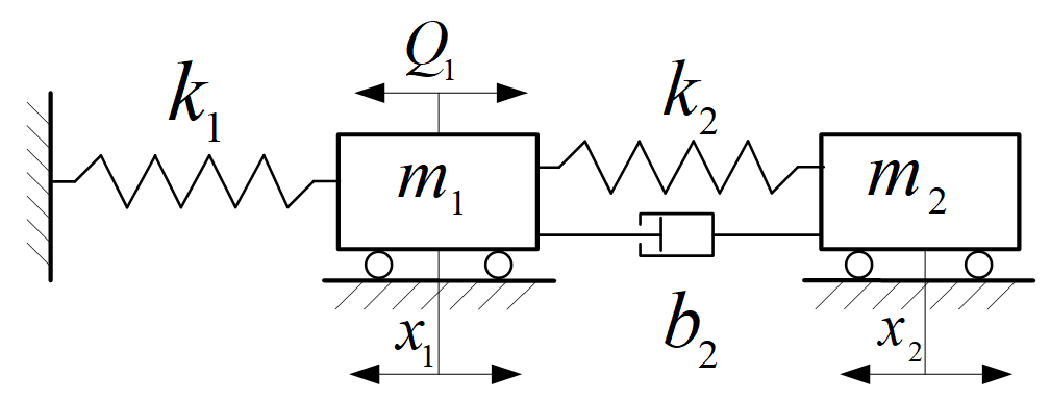
\includegraphics[width=0.7\textwidth]{den-gartog1.pdf}
		\caption{Design scheme of the mechanical oscillatory system: $m_1$ --- primary mass (vibrator), $m_2$ --- absorber mass (working organ), $k_1$, $k_2$ --- stiffness coefficients, $b_2$ --- viscous friction coefficient, $Q_1$ --- external harmonic excitation}
		\label{fig:scheme}
	\end{figure}
	
	Kinetic energy, potential energy, and dissipation function are given by:
	\begin{equation}
		T = \frac{1}{2} m_1 \dot{x}_1^2 + \frac{1}{2} m_2 (\dot{x}_2 - \dot{x}_1)^2, \quad
		\Pi = \frac{1}{2} k_1 x_1^2 + \frac{1}{2} k_2 (x_2 - x_1)^2, \quad
		\Phi = \frac{1}{2} b_2 (\dot{x}_2 - \dot{x}_1)^2.
	\end{equation}
	
	Lagrange's equations of the second kind take the form:
	\begin{equation}
		\begin{cases}
			m_1 \ddot{x}_1 + k_1 x_1 - k_2 (x_2 - x_1) - b_2 (\dot{x}_2 - \dot{x}_1) = Q(t), \\
			m_2 \ddot{x}_2 + k_2 (x_2 - x_1) + b_2 (\dot{x}_2 - \dot{x}_1) = 0.
		\end{cases}
		\label{eq:lagrange}
	\end{equation}
	
	
	Applying Laplace integral transform \cite{Lurie} to the differential equation system \eqref{eq:lagrange} yields an algebraic equation system:
	\begin{equation}
		\begin{pmatrix}
			m_1 p^2 + b_2 p + k_1 + k_2 & -(k_2 + b_2 p) \\
			-(k_2 + b_2 p) & m_2 p^2 + b_2 p + k_2
		\end{pmatrix}
		\begin{pmatrix}
			\bar{x}_1 \\
			\bar{x}_2
		\end{pmatrix}
		=
		\begin{pmatrix}
			\bar{Q}_1 \\
			0
		\end{pmatrix}
		\label{eq:laplace}
	\end{equation}
	
	Within the structural approach framework, the algebraic equation system \eqref{eq:laplace} can be represented as a structural diagram dynamically equivalent to an automatic control system structural diagram (Fig.~\ref{fig:structural}).
	
	\begin{figure}[H]
		\centering
		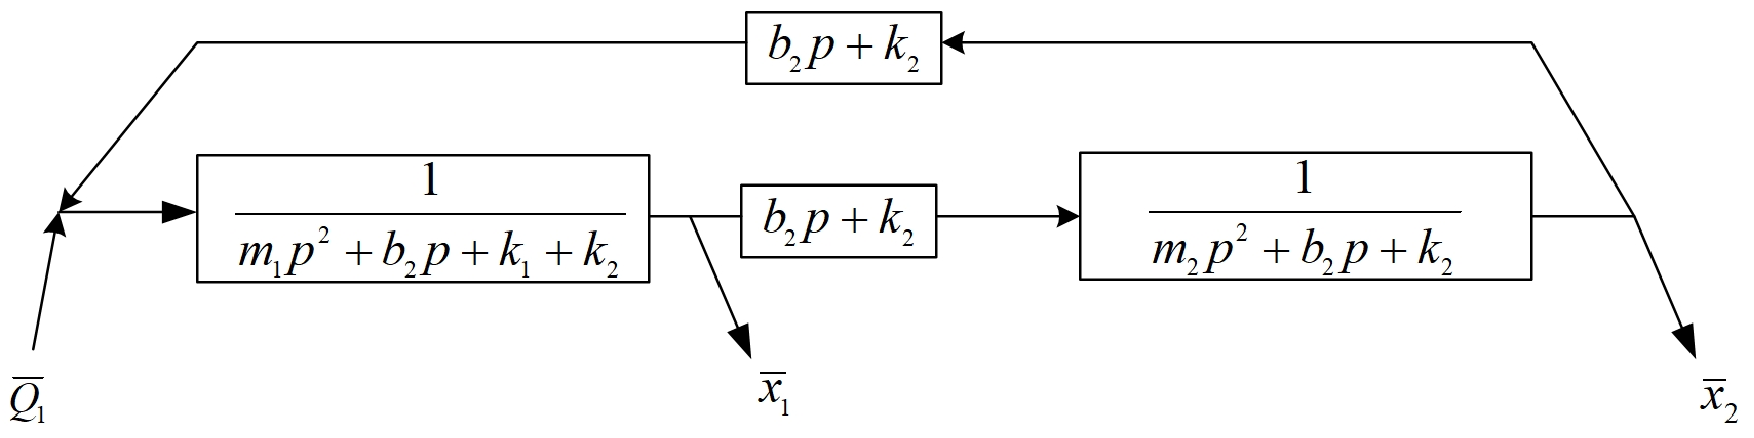
\includegraphics[width=0.9\textwidth]{figure2_structural_2dof.pdf}
		\caption{Structural diagram corresponding to the mechanical oscillatory system in Fig.~\ref{fig:scheme}: $p=j\omega$ complex variable, $j=\sqrt{-1}$ imaginary unit, $\omega$ external harmonic excitation frequency}
		\label{fig:structural}
	\end{figure}
	
	Based on the structural diagram (Fig.~\ref{fig:structural}), transfer functions representing dynamic compliance can be constructed: 	
	\begin{equation}
		W_1(p)=\frac{\bar{x}_1}{\bar{Q}_1} = \frac{m_2 p^2 + b_2 p + k_2}{A}, 
	\end{equation}
	\begin{equation}
		W_2(p)=\frac{\bar{x}_2}{\bar{Q}_1} = \frac{b_2 p + k_2}{A},
	\end{equation}
	where $A=(m_1 p^2 + b_2 p + k_1 + k_2)(m_2 p^2 + b_2 p + k_2)- (k_2 + b_2 p)^2$ is the characteristic polynomial.
	
	Alongside system transfer functions, the inter-partial connection transfer function can be considered:
	\begin{equation}
		W_{12}(p)=\frac{\bar{x}_1}{\bar{x}_2} = \frac{m_2 p^2 + b_2 p + k_2}{b_2 p + k_2}.
	\end{equation}
	The inter-partial transfer function enables evaluation of lever interaction features realized in the system depending on external excitation frequency.
	
	\section*{III. Normalized Mathematical Model}
	For mathematical model normalization, introduce dimensionless variables:
	\begin{equation}
		\mu = \frac{m_2}{m_1},\quad
		\Omega_c = \sqrt{\frac{k_1}{m_1}},\quad
		f = \frac{\omega_a}{\Omega_c},\quad
		g = \frac{\omega}{\Omega_c},\quad
		\gamma = \frac{b_2}{2 m_2 \Omega_c},
		\label{eq:nondim}
	\end{equation}
	where $\omega_a = \sqrt{k_2/m_2}$ is the absorber's partial frequency, $\omega$ is the external harmonic excitation frequency. Transforming algebraic system \eqref{eq:laplace} to dimensionless variables \eqref{eq:nondim} yields the matrix form:
	\begin{equation}
		(\mathbf{M}_{Re} + j \mathbf{M}_{Im}) \cdot \mathbf{X}^* = \mathbf{F}^*,
		\label{eq:matrix}
	\end{equation}
	where $\mathbf{X}^{*}$ is the image vector, $\mathbf{F}^{*}$ is the right-hand side vector, $\mathbf{M}_{Re}$ is the real part and $\mathbf{M}_{Im}$ the imaginary part of complex dynamic stiffness matrix $\mathbf{M}$ from \eqref{eq:laplace}:
	\begin{align}
		\mathbf{M}_{Re} &= 
		\begin{bmatrix}
			\mu f^2 - g^2 + 1 & -\mu f^2 \\
			-\mu f^2 & \mu f^2 - \mu g^2
		\end{bmatrix},
		\label{eq:MR} \\
		\mathbf{M}_{Im} &= 
		\begin{bmatrix}
			2\gamma\mu g & -2\gamma\mu g \\
			-2\gamma\mu g & 2\gamma\mu g
		\end{bmatrix},
		\label{eq:MI} \\
		\mathbf{X}^{*} &= 
		\begin{bmatrix}
			X^{*}_1 \\
			X^{*}_2
		\end{bmatrix},\quad
		\mathbf{F}^{*} = 
		\begin{bmatrix}
			1 \\
			0
		\end{bmatrix}.
	\end{align}
	
	Normalized transfer functions take the form:
	
	\begin{equation}
		|\mathbf{X}^{*}_{1}| = \frac{\left|\det\left(
			\begin{bmatrix}
				1 & -\mu f^{2} \\
				0 & \mu f^{2} - \mu g^{2}
			\end{bmatrix}
			+
			\begin{bmatrix}
				1 & -2\mathrm{j}\gamma\mu g \\
				0 & 2\mathrm{j}\gamma\mu g
			\end{bmatrix}
			\right)\right|}{|\det\mathbf{M}|},
	\end{equation}
	
	\begin{equation}
		|\mathbf{X}^{*}_{2}| = \frac{\left|\det\left(
			\begin{bmatrix}
				\mu f^2 - g^2 + 1 & 1 \\
				-\mu f^2 & 0
			\end{bmatrix}
			+
			\begin{bmatrix}
				2 j\gamma\mu g & 1 \\
				-2 j \gamma\mu g & 0
			\end{bmatrix}
			\right)\right|}{|\det\mathbf{M}|},
	\end{equation}
	
	
	\begin{equation}
		\frac{|\mathbf{X}^{*}_{1}|}{	|\mathbf{X}^{*}_{2}|} = \frac{\left|\det\left(
			\begin{bmatrix}
				1 & -\mu f^{2} \\
				0 & \mu f^{2} - \mu g^{2}
			\end{bmatrix}
			+
			\begin{bmatrix}
				1 & -2\mathrm{j}\gamma\mu g \\
				0 & 2\mathrm{j}\gamma\mu g
			\end{bmatrix}
			\right)\right|}
		{\left|\det\left(
			\begin{bmatrix}
				\mu f^2 - g^2 + 1 & 1 \\
				-\mu f^2 & 0
			\end{bmatrix}
			+
			\begin{bmatrix}
				2 j\gamma\mu g & 1 \\
				-2 j \gamma\mu g & 0
			\end{bmatrix}
			\right)\right|},
	\end{equation}
	
	
	
	where determinant of complex stiffness matrix $\mathbf{M}=\mathbf{M}_{Re}+j\mathbf{M}_{Im}$ is:
	\begin{align}
		\det \mathbf{M} &= \Delta_{Re} + j \Delta_{Im},
		\label{eq:determinant} \\
		\Delta_{Re} &= -\mu^2 f^2 g^2 - \mu f^2 g^2 + \mu g^4 + \mu f^2 - \mu g^2,
		\label{eq:DeltaR} \\
		\Delta_{Im} &= -2\gamma\mu^2 g^3 - 2\gamma\mu g^3 + 2\gamma\mu g.
		\label{eq:DeltaI}
	\end{align}
	
	We use notations $A_1^2(g)=|\mathbf{X}^{*}_{1}|^2$ and $A_2^2(g)=|\mathbf{X}^{*}_{2}|^2$, where $A_1^2(g)$ and $A_2^2(g)$ are squares of amplitude-frequency characteristics expressed using dimensionless parameters, considered as functions of dimensionless frequency $g$.
	
	\section*{IV. Features of Normalized Amplitude-Frequency Characteristic of System $A_1$}
	
	Square of dimensionless amplitude of forced oscillations of generalized coordinate $\mathbf{X^{*}_{1}}$ $m_1$ is given by:
	\begin{equation}
		A_1^2(g) = \frac{(2\gamma\mu g)^2 + [\mu(f^2 - g^2)]^2}{
			[2g\gamma\mu(-g^2\mu - g^2 + 1)]^2 + 
			[-f^2g^2\mu^2 - f^2g^2\mu + g^4\mu + \mu f^2 - \mu g^2]^2
		}.
		\label{eq:A1}
	\end{equation}
	
	It is known that families of amplitude-frequency characteristics considered as functions of viscous friction coefficient $\gamma$ have so-called nodal points through which every amplitude-frequency characteristic of the family passes \cite{DenHartog1956}. Nodal points of amplitude-frequency characteristic families are independent of viscous friction coefficient and are used for forming dynamic quality of mechanical oscillatory systems.    
	
	To determine nodal points, construct amplitude-frequency characteristics for two limiting values of viscous friction coefficients $\gamma \to 0$ and $\gamma \to \infty$:
	\begin{align}
		|A_1|_{\gamma \to 0} &= \left| \frac{f^2 - g^2}{-g^4 + (1 + (\mu+1)f^2)g^2 - f^2} \right|,
		\label{eq:A1_gamma0} \\
		|A_1|_{\gamma \to \infty} &= \left| \frac{1}{-1 + (\mu+1)g^2} \right|.
		\label{eq:A1_gammainf}
	\end{align}
	
	
	Intersection of amplitude-frequency characteristic graphs for limiting $\gamma$ values $|A_1|_{\gamma \to 0} = |A_1|_{\gamma \to \infty}$ allows determination of nodal points---frequencies where amplitude $|A_1|$ is independent of friction coefficient $\gamma$. Frequencies determining nodal points are found from the biquadratic equation in frequency $g$:
	
	\begin{equation}
		(\mu+2) g^4 - 2\bigl((\mu+1)f^2 + 1\bigr) g^2 + 2f^2 = 0.
		\label{eq:biquadratic_A1}
	\end{equation}
	
	Roots of equation \eqref{eq:biquadratic_A1} are:
	\begin{equation}
		g_{1,2}^2 = \frac{f^2(\mu+1)+1}{\mu+2} \pm 
		\sqrt{\frac{f^4\mu}{\mu+2} + \left(\frac{f^2-1}{\mu+2}\right)^2}.
		\label{eq:g12_general}
	\end{equation}
	Corresponding amplitude-frequency characteristic values are:
	\begin{equation}
		|A_1(g_1)| = \left| \frac{-\mu -2}{\left(-\mu -1\right) \sqrt{1+\left(\mu +1\right)^{2} f^{4}-2 f^{2}}+f^{2} \mu^{2}+2 \mu f^{2}+f^{2}-1} \right|,
	\end{equation}
	\begin{equation}
		|A_1(g_2)| = \left| \frac{-\mu -2}{\left(\mu + 1\right) \sqrt{1+\left(\mu +1\right)^{2} f^{4}-2 f^{2}}+f^{2} \mu^{2}+2 \mu f^{2}+f^{2}-1} \right|.
	\end{equation}
	
	Presented roots~\eqref{eq:g12_general} and amplitude-frequency characteristic values form so-called nodes independent of system friction. Such nodes are of interest for forming dynamic features of resonant modes. Frequencies determining intersection nodal points of amplitude-frequency characteristics play a key role precisely because their frequency position and amplitude level remain unchanged under any variations of system damping coefficient. This feature enables construction of dynamic system behavior based on stiffness and inertial tuning while ensuring the beneficial effect won't be destroyed by inevitable technological scatter of dissipative parameters or their changes during operation. In practice, nodal points are used for forming dynamic quality of resonant modes: for example, equalizing nodal heights creates a so-called "plateau" on the amplitude-frequency characteristic near resonance, minimizing amplitude sensitivity to damping detuning, while amplitude reduction between nodes ensures vibration absorption \cite{Eliseev2017}. Additionally, independence of inter-partial transfer function from friction at a specific point enables dynamic property estimation without precise knowledge of friction, potentially enhancing technical condition monitoring reliability.
	
	One approach to forming system dynamic properties is determining conditions ensuring nodes are aligned at the same height \cite{DenHartog1956}. Basic conditions of equal amplitude-frequency characteristic values at nodal points
	\begin{equation}
		|A_1(g_1)| = |A_1(g_2)| 
	\end{equation} 
	lead to explicit dependence between mass coefficient and frequency ratio $f$:
	\begin{equation}
		f = \frac{1}{1+\mu}.
		\label{eq:f_opt1}
	\end{equation}
	
	Under basic conditions of equal ordinates (heights) of amplitude-frequency characteristics, nodal frequency values are:
	\begin{equation}
		g_{1}^2 = \frac{1}{1+\mu}\left(1 - \sqrt{\frac{\mu}{\mu+2}}\right),
	\end{equation}		
	\begin{equation}		
		g_{2}^2 = \frac{1}{1+\mu}\left(1 + \sqrt{\frac{\mu}{\mu+2}}\right).
		\label{eq:g12_opt} \\
	\end{equation}
	
	Corresponding common amplitude-frequency characteristic height at nodal frequencies is:
	\begin{equation}
		|A_{1,eq}(g_{1,2})| = \sqrt{\frac{\mu+2}{\mu}}.
		\label{eq:H1_opt}
	\end{equation}
	
	However, equal amplitude-frequency characteristic conditions at nodal frequencies don't ensure optimal shape in the interval between nodal frequencies. To select optimal amplitude-frequency characteristic shape, a dynamic state quality criterion depending on friction coefficient $\gamma$ must be specified. One approach to selecting optimal amplitude-frequency characteristic shape involves energy norm minimization problems reflecting dynamic quality features of vibrational system states \cite{Nishihara2002}. However, this approach may lack clear analytical solutions. The solution is determining optimal friction from three-point equality conditions: adding a requirement for amplitude-frequency characteristic value at some intermediate frequency (e.g., equidistant from nodal frequencies) to the two-nodal equality condition. This approach enables determination of three-point "plateau" amplitude-frequency characteristic ensuring more stable operation of corresponding vibrational technological machine elements in the frequency range between nodal frequencies. 
	
	\section*{V. Selection of Damping Coefficient for Three-Point Plateau Implementation}
	
	Conditions for three-point "plateau" implementation constitute a system of paired amplitude-frequency characteristic equalities at three frequencies: 
	\begin{equation}
		A_1(g_1) = A_1(g_0) = A_1(g_2),
		\label{eq:gamma_cr}
	\end{equation}
	where $g_0 = \frac{1}{\sqrt{1+\mu}}$ serves as intermediate point between frequencies $g_1$ and $g_2$. Solving equations for friction coefficient $\gamma$ yields critical friction coefficient \eqref{eq:gamma_cr}:
	\begin{equation}
		\gamma_{\text{cr}}^{2} = \frac{\mu}{2 \left(\mu +1\right)^{3}}.
	\end{equation}
	
	This value uniquely determines final amplitude-frequency characteristic shape, eliminating dynamic quality adjustment possibility. However, there might be a need either to intensify oscillation levels or, conversely, reduce oscillation amplitudes. 
	
	To account for dynamic quality requirements, consider determining friction coefficient from conditions allowing oscillation amplitude intensification/reduction at intermediate frequency $g_0$:
	\begin{equation}
		A_1(g_1)(1+\varepsilon) = A_1(g_0) = A_1(g_2)(1+\varepsilon),
	\end{equation}
	where $\varepsilon$ is oscillation mode amplification/attenuation coefficient, $\varepsilon > 0$ indicates oscillation intensification, $\varepsilon < 0$ indicates oscillation attenuation. Considering intensity coefficient $\varepsilon$, corresponding viscous friction coefficient becomes:
	\begin{equation}
		\gamma^{2}_{\text{opt}} (\varepsilon) = \frac{\mu }{2 \left(\mu  +1\right)^{3}} + \varepsilon \frac{\mu \left(\mu +2\right)}{2 \left(\mu +1\right)^{3}} +\varepsilon^{2} \frac{\mu\left(\mu +2\right)}{4 \left(\mu+1\right)^{3}}.
	\end{equation}
	
	If $\varepsilon=0$, a three-point conditional "plateau" is implemented. Figure~\ref{fig:a1_mu1} shows amplitude-frequency characteristic family for fixed coefficient $\mu=0.1$ (i.e., considering dynamic resonance mode absorption model where mass $m_1$ serves as primary mass and auxiliary mass $m_1$ as dynamic absorber). Figure~\ref{fig:a1_mu1} shows all curves $|A_1(g)|$ intersect at two nodes with coordinates independent of coefficient $\gamma$. 
	
	\begin{figure}[H]
		\centering
		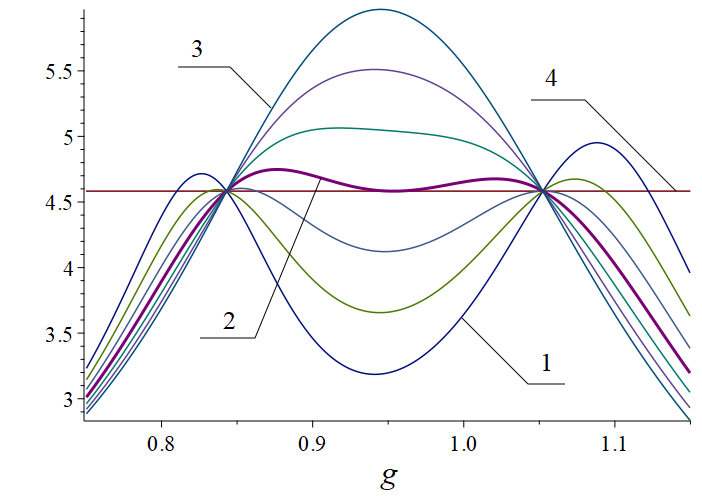
\includegraphics[width=0.8\textwidth]{a1gamma.png}
		\caption{Amplitude-frequency characteristics $|A_1(g)|$ for dynamic absorber mode ($\mu = 0.1$, $f = 0.91$). Curve family defined by friction coefficients $\gamma(\varepsilon)$, where $\varepsilon = -0.02 .. 0.02, 0.01$; line 1 --- $\varepsilon = -0.02$, line 2 --- $\varepsilon = 0$ (plateau), line 1 --- $\varepsilon = 0.02$, line 4 --- level $\sqrt{\frac{\mu+2}{\mu}} $}
		\label{fig:a1_mu1}
	\end{figure}
	
	Specifically, for damping coefficients $\gamma_{\text{cr}}$ corresponding to parameters $\varepsilon = -0.02 .. 0.02, 0.01$, amplitude-frequency characteristics passing through two nodal points are constructed. Line 1 shows oscillation amplitude reduction mode; line 3 --- amplitude increase; three-point plateau is shown by line 2 with critical damping, having height at intermediate frequency $g_0$ matching amplitude-frequency characteristic values at nodal frequencies $g_1$ and $g_2$.
	
	Alongside vibrator absorber model, vibrator test stand model can be considered, where mass $m_2$ (working organ) is significantly larger than mass $m_1$ (vibrator). Figure~\ref{fig:a1_mu01} shows example for $\mu = 10$ amplitude-frequency characteristics differing from those in Fig.~\ref{fig:a1_mu1} by extremely asymmetric plateau shape skewed leftward; however, critical amplitude-frequency characteristic proximity to constant value is sufficiently pronounced. 
	
	\begin{figure}[H]
		\centering
		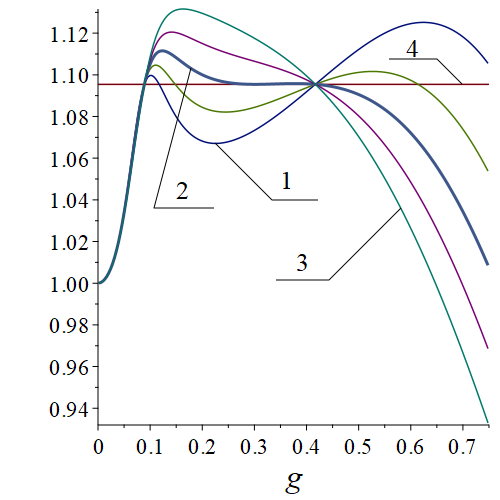
\includegraphics[width=0.8\textwidth]{a1mu10gamma}
		\caption{Amplitude-frequency characteristic family $|A_1(g)|$ for fixed coefficient $\mu = 10$ with various damping coefficients $\gamma(\varepsilon)$, where $\varepsilon = -0.02 .. 0.02, 0.01$; line 1 --- $\varepsilon = -0.02$, line 2 --- $\varepsilon = 0$, line 1 --- $\varepsilon = 0.02$, line 4 --- level $\sqrt{\frac{\mu+2}{\mu}} $}				
		\label{fig:a1_mu01}
	\end{figure}
	
	
	Figure~\ref{fig:A1_platoA1} shows dependency forms of amplitude-frequency characteristic $A_1$ values on coefficient $\mu$. 
	
	
	\begin{figure}[H]
		\centering
		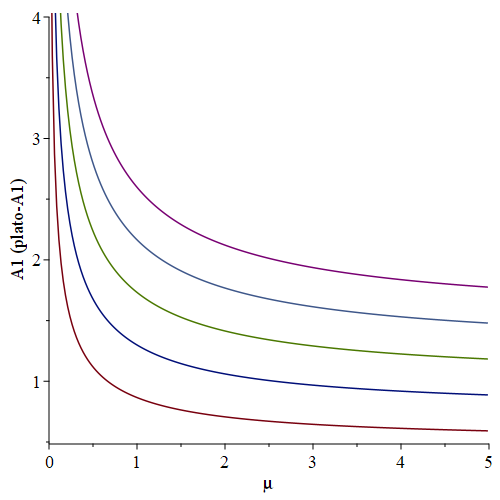
\includegraphics[width=0.8\textwidth]{A1_platoA1.png}
		\caption{Amplitude-frequency characteristic values $A_2(g_0)$ for $\varepsilon = -0.5 .. 0.5, 0.25$: line 1 reaches zero value for some critical $\mu$, lines 2 and 3 don't vanish}
		\label{fig:A1_platoA1}
	\end{figure}	
	
	Specifically, for $\varepsilon$ set, increasing coefficient $\mu$ reduces generalized coordinate oscillation amplitude. Graphs show that as mass coefficient $\mu$ increases, three-point plateau vertical magnitude decreases, while decreasing $\mu$ increases it.
	
	Figure~\ref{fig:A2_platoA1} shows dependency of amplitude-frequency characteristic $A_2$ values on coefficient $\mu$. Key difference is existence of critical mass ratio $\mu$ where amplitude-frequency characteristic values at frequency $g_0$ vanish. 
	
	Meanwhile, amplitude $A_2$ of generalized coordinate $X_2$ monotonically decreases. However, $A_2$ amplitude decay character differs for various $\varepsilon$ values. Specifically, there exists critical mass coefficient $\mu$ where $A_2(g_0)=0$.
	
	\begin{figure}[h]
		\centering
		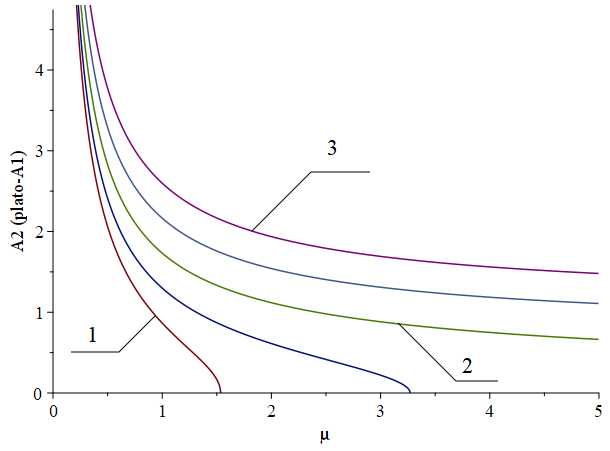
\includegraphics[width=0.8\textwidth]{A2_platoA1.png}
		\caption{Amplitude-frequency characteristic family values. $\varepsilon = -0.5 .. 0.5, 0.25$} depending on mass coefficient $\mu$
		\label{fig:A2_platoA1}
	\end{figure}
	
	Meanwhile, changing mass coefficient $\mu$ alters nodal frequency positions $g_1$, $g_2$, and intermediate frequency (between nodal frequencies) $g_0$.
	
	Figure~\ref{fig:Eq_tochki_plato_A1} shows nodal frequency coordinates for amplitude-frequency characteristic implementing three-point plateau.
	
	\begin{figure}[H]
		\centering
		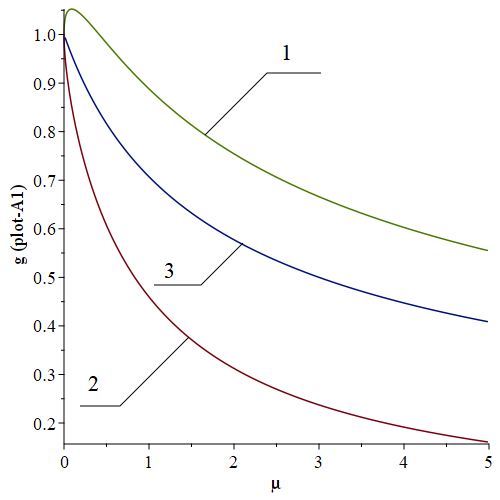
\includegraphics[width=0.8\textwidth]{Eq_tochki_plato_A1.png}
		\caption{Nodal frequencies $g_1$, $g_2$ and intermediate point $g_0$ depending on mass ratio coefficient $\mu$. 1,2 --- nodal frequency points, 3 --- intermediate frequency $g_0$ }
		\label{fig:Eq_tochki_plato_A1}
	\end{figure}	
	
	
	Note that distance between nodal frequencies depends on mass coefficient $\mu$. Figure~\ref{fig:extrem_A1_mu1} shows graph of difference between nodal frequencies. Key feature is that internal global maximum is achieved for nodal frequency difference function.
	
	
	\begin{figure}[H]
		\centering
		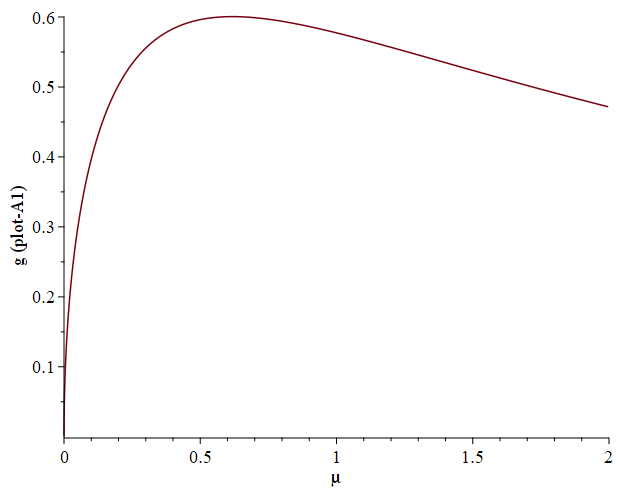
\includegraphics[width=0.8\textwidth]{extrem_A1_mu1.png}
		\caption{Distance between nodes $g_1$, $g_2$ and intermediate point $g_0$ depending on mass ratio coefficient $\mu$. }
		\label{fig:extrem_A1_mu1}
	\end{figure}
	
	Figure~\ref{fig:extrem_A1_mu1} shows distances between nodal points as functional dependency on independent variable $\mu$. Coefficient $\mu$ providing maximum distance between nodal frequencies can be determined analytically. Specifically, for coefficient $\mu = \frac{\sqrt{5}}{2}-\frac{1}{2}$ maximum frequency distance is:
	
	\begin{equation}
		\Delta g^2 =\frac{2 \sqrt{\sqrt{5}-1}\, \sqrt{2}}{\sqrt{5}+3} = 0.6005662114.
	\end{equation}
	
	Amplitude-frequency characteristic $A_1$ value for parameter $\mu$ providing maximally wide distance between nodal points is: 
	
	\begin{equation}
		A_1 = \frac{\sqrt{2}\, \left(\sqrt{5}+1\right)}{2 \sqrt{\sqrt{5}-1}} = 2.058171028.
	\end{equation}
	
	Amplitude-frequency characteristic $A_2$ value is:
	
	\begin{equation}
		A_2 = \frac{2 \,5^{{1}/{4}}}{\sqrt{5}-1} =2.419525154.
	\end{equation}
	
	Corresponding amplitude-frequency characteristics are shown in Fig.\ref{fig:trig_platoA1}.	
	
	\begin{figure}[H]
		\centering
		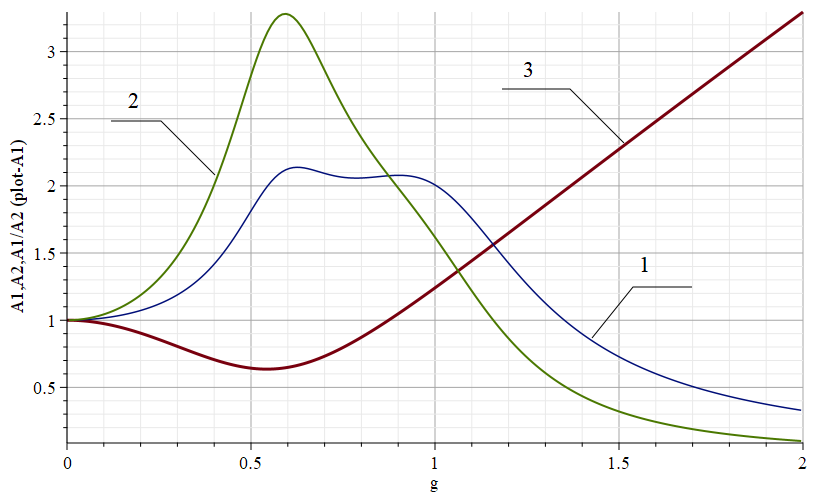
\includegraphics[width=0.8\textwidth]{trig_platoA1.png}
		\caption{Reference amplitude-frequency characteristics: 1 --- partial system $X_1$ amplitude-frequency characteristic, 2 --- $X_2$, 3 --- inter-partial system $X_1/X_2$}
		\label{fig:trig_platoA1}
	\end{figure}
	
	Thus, amplitude-frequency characteristics and parameters ensuring maximum distance between nodal frequencies can be determined, enabling introduction of reference vibrational system. This system serves as reference for analysis and synthesis of mechanical oscillatory systems.
	
	
	\section*{VI. Dependency of Amplitude-Frequency Characteristic Forms for System Implementing Three-Point $A_1$-Plateau Conditions}	
	
	Below are amplitude-frequency characteristics constructed for various parameter values $0<\mu<1$ (Fig.~\ref{fig:A1_01}--\ref{fig:A1_10}).
	
	\begin{figure}[H]
		\centering
		\begin{minipage}{0.45\textwidth}
			\centering
			\includegraphics[width=\textwidth]{platoA1mu01.eps}
			\caption{\(\mu = 0.1\)}
			\label{fig:A1_01}
		\end{minipage}\hfill
		\begin{minipage}{0.45\textwidth}
			\centering
			\includegraphics[width=\textwidth]{platoA1mu02.eps}
			\caption{\(\mu = 0.2\)}
			\label{fig:A1_02}
		\end{minipage}
	\end{figure}
	
	\begin{figure}[H]
		\centering
		\begin{minipage}{0.45\textwidth}
			\centering
			\includegraphics[width=\textwidth]{platoA1mu03.eps}
			\caption{\(\mu = 0.3\)}
			\label{fig:A1_03}
		\end{minipage}\hfill
		\begin{minipage}{0.45\textwidth}
			\centering
			\includegraphics[width=\textwidth]{platoA1mu04.eps}
			\caption{\(\mu = 0.4\)}
			\label{fig:A1_04}
		\end{minipage}
	\end{figure}
	
	\begin{figure}[H]
		\centering
		\begin{minipage}{0.45\textwidth}
			\centering
			\includegraphics[width=\textwidth]{platoA1mu05.eps}
			\caption{\(\mu = 0.5\)}
			\label{fig:A1_05}
		\end{minipage}\hfill
		\begin{minipage}{0.45\textwidth}
			\centering
			\includegraphics[width=\textwidth]{platoA1mu06.eps}
			\caption{\(\mu = 0.6\)}
			\label{fig:A1_06}
		\end{minipage}
	\end{figure}
	
	\begin{figure}[H]
		\centering
		\begin{minipage}{0.45\textwidth}
			\centering
			\includegraphics[width=\textwidth]{platoA1mu07.eps}
			\caption{\(\mu = 0.7\)}
			\label{fig:A1_07}
		\end{minipage}\hfill
		\begin{minipage}{0.45\textwidth}
			\centering
			\includegraphics[width=\textwidth]{platoA1mu08.eps}
			\caption{\(\mu = 0.8\)}
			\label{fig:A1_08}
		\end{minipage}
	\end{figure}
	
	\begin{figure}[H]
		\centering
		\begin{minipage}{0.45\textwidth}
			\centering
			\includegraphics[width=\textwidth]{platoA1mu09.eps}
			\caption{\(\mu = 0.9\)}
			\label{fig:A1_09}
		\end{minipage}\hfill
		\begin{minipage}{0.45\textwidth}
			\centering
			\includegraphics[width=\textwidth]{platoA1mu10.eps}
			\caption{\(\mu = 1.0\)}
			\label{fig:A1_10}
		\end{minipage}
	\end{figure}
	
	
	Key feature of amplitude-frequency characteristics $A_1$, $A_2$ and $A_{12}$ shown in Fig.~\ref{fig:A1_01}--\ref{fig:A1_10} is amplitude reduction as coefficient $\mu$ increases.
	
	Significant increase of coefficient $\mu>>1$ causes "plateau" region value for amplitude-frequency characteristic $A_1$ of first coordinate $X_1$ to approach unity, while resonance frequency (frequency achieving local maximum) for coordinate $X_2$ shifts toward origin. These features are shown in Fig.~\ref{fig:A1_mu10}--\ref{fig:A1_mu100}. 
	
	Practical significance of these features manifests in systems operating in primary mass $m_1$ oscillation absorption mode, which may be accompanied by either increased absorber oscillation amplitudes or decreased oscillation amplitudes. Achieving primary mass oscillation reduction effect leads to coincidence of oscillation amplitudes for both primary mass and absorber mass.  
	
	\begin{figure}[H]
		\centering
		\begin{minipage}{0.45\textwidth}
			\centering
			\includegraphics[width=\textwidth]{platoA1_mu10.eps}
			\caption{\(\mu = 10\)}
			\label{fig:A1_mu10}
		\end{minipage}\hfill
		\begin{minipage}{0.45\textwidth}
			\centering
			\includegraphics[width=\textwidth]{platoA1_mu20.eps}
			\caption{\(\mu = 20\)}
			\label{fig:A1_mu20}
		\end{minipage}
	\end{figure}
	
	\begin{figure}[H]
		\centering
		\begin{minipage}{0.45\textwidth}
			\centering
			\includegraphics[width=\textwidth]{platoA1_mu30.eps}
			\caption{\(\mu = 30\)}
			\label{fig:A1_mu30}
		\end{minipage}\hfill
		\begin{minipage}{0.45\textwidth}
			\centering
			\includegraphics[width=\textwidth]{platoA1_mu40.eps}
			\caption{\(\mu = 40\)}
			\label{fig:A1_mu40}
		\end{minipage}
	\end{figure}
	
	\begin{figure}[H]
		\centering
		\begin{minipage}{0.45\textwidth}
			\centering
			\includegraphics[width=\textwidth]{platoA1_mu50.eps}
			\caption{\(\mu = 50\)}
			\label{fig:A1_mu50}
		\end{minipage}\hfill
		\begin{minipage}{0.45\textwidth}
			\centering
			\includegraphics[width=\textwidth]{platoA1_mu60.eps}
			\caption{\(\mu = 60\)}
			\label{fig:A1_mu60}
		\end{minipage}
	\end{figure}
	
	\begin{figure}[H]
		\centering
		\begin{minipage}{0.45\textwidth}
			\centering
			\includegraphics[width=\textwidth]{platoA1_mu70.eps}
			\caption{\(\mu = 70\)}
			\label{fig:A1_mu70}
		\end{minipage}\hfill
		\begin{minipage}{0.45\textwidth}
			\centering
			\includegraphics[width=\textwidth]{platoA1_mu80.eps}
			\caption{\(\mu = 80\)}
			\label{fig:A1_mu80}
		\end{minipage}
	\end{figure}
	
	\begin{figure}[H]
		\centering
		\begin{minipage}{0.45\textwidth}
			\centering
			\includegraphics[width=\textwidth]{platoA1_mu90.eps}
			\caption{\(\mu = 90\)}
			\label{fig:A1_mu90}
		\end{minipage}\hfill
		\begin{minipage}{0.45\textwidth}
			\centering
			\includegraphics[width=\textwidth]{platoA1_mu100.eps}
			\caption{\(\mu = 100\)}
			\label{fig:A1_mu100}
		\end{minipage}
	\end{figure}
	
	
	Models corresponding to $\mu >> 1$ reflect dynamic features of vibrational technological machine oscillations. Specifically, it can be stated that vibrator $m_1$ reaching three-point plateau initially increases working organ oscillation amplitudes, but during acceleration reduces working organ oscillation amplitudes.
	
	
	
	Intersection point is shown in Fig.~\ref{fig:perA1A2platoA1}. 
	
	
	\begin{figure}[H]
		\centering
		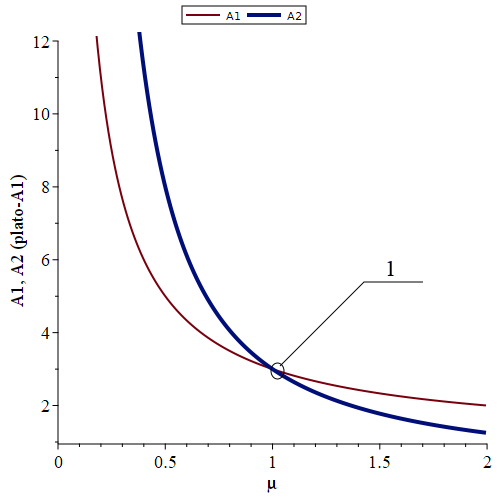
\includegraphics[width=0.8\textwidth]{perA1A2platoA1.png}
		\caption{Curve intersection allows finding critical mass ratio $\mu=1$}
		\label{fig:perA1A2platoA1}
	\end{figure}
	
	Analytical relation $\mu=1$ can be found from equation:	
	
	\begin{equation}
		\frac{\mu+2}{\mu} = 
		\frac{2 \mu+1}{\mu^{2}}.
	\end{equation}	
	
	Overall, first coordinate reaching "plateau" is accompanied by simultaneous second coordinate reaching resonance (oscillation amplitude increase, $\mu<1$), or prior resonance transition with subsequent frequency approach to origin ($\mu >> 1$).
	
	Thus, mass ratio coefficient is key factor in forming "plateau" level or height of first generalized coordinate amplitude-frequency characteristic, representing oscillations of concentrated mass $m_1$ subjected to harmonic force excitation.
	
	Alongside dynamic quality of first coordinate oscillations related to $m_1$, dynamic quality analysis of second coordinate related to $m_2$ can be conducted.
	
	\section*{VII. Features of Nodal Frequency Formation for System Amplitude-Frequency Characteristic $A_2$}	
	
	To evaluate dynamic states related to forced oscillations of mass $m_2$ under disturbing force $Q_1$, consider dimensionless amplitude-frequency characteristic $A_2$ of transfer function $W_2$:
	
	\begin{equation}
		A_2^2(g) = \frac{f^4\mu^2 + 4\gamma^2\mu^2 g^2}{
			[-2g^3\gamma\mu(\mu+1)+2\gamma\mu g]^2 + 
			[-f^2g^2\mu(\mu+1)+g^4\mu+\mu f^2-\mu g^2]^2
		}.
		\label{eq:A2}
	\end{equation}
	
	Use known nodal point determination method \cite{DenHartog1956}. Specifically, nodes of amplitude-frequency characteristic family \eqref{eq:A2} are considered as intersection points of two amplitude-frequency characteristic graphs for limiting values $\gamma=0$ and $\gamma=\infty$:	
	
	\begin{align}
		|A_2|_{\gamma \to 0} &= \frac{\mu f^2}{|g^4 - (1+(\mu+1)f^2)g^2 + f^2|},
		\label{eq:A2_gamma0} \\
		|A_2|_{\gamma \to \infty} &= \frac{1}{|1 - (\mu+1)g^2|}.
		\label{eq:A2_gammainf}
	\end{align}
	
	Condition for frequencies $g$ where amplitude-frequency characteristic graphs intersect, 
	
	\begin{equation}
		|A_2(g)|_{\gamma \to 0} = |A_2(g)|_{\gamma \to \infty} 
	\end{equation}	
	
	leads to algebraic equations whose roots determine nodal frequencies:
	
	\begin{align}
		g^4 - g^2 &= 0,\\
		g^4 - \bigl(2(\mu+1)f^2 + 1\bigr) g^2 + 2f^2 &= 0.
	\end{align}
	Non-trivial equation solutions are:
	\begin{equation}
		g_{l,r}^2 = f^2(1+\mu) + \frac{1}{2} \pm \frac{1}{2}\sqrt{4f^4(1+\mu)^2 + 4f^2(\mu-1) + 1},\quad
		g_c^2 = 1.
		\label{eq:tritochki}
	\end{equation}
	
	Solution is determined by graph intersection at three nodal points defining three frequencies: $g_l$ --- "left", $g_c = 1$ --- "central", $g_r$ --- "right". Height at central node $g_c$ is:
	\begin{equation}
		|A_2(g_c)| = \frac{1}{\mu}.
		\label{eq:Hc}
	\end{equation}
	
	Amplitude-frequency characteristic values at nodes $g_l$ and $g_r$ are given by:
	\begin{align}
		A_2(g_l) &= \frac{-2 f^{2} \mu^{2}-4 \mu f^{2}-2 f^{2}-\mu+1-\sqrt{1+4 \left(\mu +1\right)^{2} f^{4}+\left(4 \mu-4\right) f^{2}}\, \left(\mu+1\right)}{2 \mu}, \\
		A_2(g_r) &= \frac{-2 f^{2} \mu^{2}-4 \mu f^{2}-2 f^{2}-\mu+1+\sqrt{1+4 \left(\mu +1\right)^{2} f^{4}+\left(4 \mu-4\right) f^{2}}\, \left(\mu+1\right)}{2 \mu}.
	\end{align}
	
	For three points~\eqref{eq:tritochki}, three conditions of pairwise amplitude-frequency characteristic equality at corresponding nodal points can be considered. Specifically, first equality $A_2(g_l)=A_2(g_c)$ implies dependence between $f$ and $\mu$:
	
	\begin{equation}
		f^2 = \frac{1-\mu}{(1+\mu)^2}, \quad 0 < \mu \le 1.
		\label{eq:f2_lc}
	\end{equation}
	
	Under condition~\eqref{eq:f2_lc}, nodal frequency values~\eqref{eq:tritochki} become:
	\begin{equation}
		g_l^2 = \frac{1-\mu}{1+\mu}, \quad 
		g_c^2 = 1, \quad 
		g_r^2 = \frac{2}{1+\mu}.
	\end{equation}
	Corresponding amplitude-frequency characteristic height (ordinates) values $A_2$ are:
	\begin{equation}
		A_2(g_l) = \frac{1}{\mu}, \quad A_2(g_c) = \frac{1}{\mu}, \quad A_2(g_r) = 1.
	\end{equation}
	
	Second amplitude coincidence condition $A_2(g_l)=A_2(g_r)$ at frequencies $g_l$, $g_r$ respectively defines dependence between $f$ and $\mu$:
	\begin{equation}
		f^2 = \frac{1-\mu}{2(\mu+1)^2}, \quad 0 \le \mu \le 1.
		\label{eq:f2_lr}
	\end{equation}
	
	Under condition \eqref{eq:f2_lr}, critical nodal point frequencies take values:
	\begin{equation}
		g_l^2 = \frac{1-\sqrt{\mu}}{1+\mu}, \quad
		g_c^2 = 1, \quad
		g_r^2 = \frac{1+\sqrt{\mu}}{1+\mu}.
	\end{equation}
	Corresponding amplitude-frequency characteristic values at nodal points are:
	\begin{equation}
		A_2(g_l) = \frac{1}{\sqrt{\mu}}, \quad 
		A_2(g_c) = \frac{1}{\mu}, \quad 
		A_2(g_r) = \frac{1}{\sqrt{\mu}}.
	\end{equation}
	
	Third condition $A_2(g_c) = A_2(g_r)$ has no solution for $\mu>0$. Therefore, equalizing ordinates of right and central nodal points $A_2$ is impossible.
	
	Among considered conditions, plateau formation question is of interest---amplitude-frequency characteristic with gentle shape in specific frequency range, particularly near resonance. Central pair frequencies $g_l$ and $g_r$ are too far apart, meaning resonance frequency may appear between them.  
	For right pair frequencies $g_{c}$, $g_r$, amplitude-frequency characteristic $A_2$ equality conditions are absent. Thus, plateau formation possibility should only be considered for left pair $g_l$ and $g_{c}$.
	
	\section*{VIII. Selection of Three-Point Plateau Parameters for Amplitude-Frequency Characteristic $A_2$}  
	
	
	By selecting friction coefficient $\gamma$, amplitude-frequency characteristic contact between $g_l$ and $g_c$ at level $A_2(g_l) = A_2(g_c)$ can be achieved at intermediate point $g_{1/2}$. 
	
	
	As intermediate frequency, consider $g_{1/2}^2=(g_l^2+g_c^2)/2$ and determine coefficient $\gamma_{1/2}$ ensuring amplitude-frequency characteristic coincidence at frequency $g_{1/2}$ with value $A_2(g_l)$.
	
	Dependency of nodal frequency values $g_l$, $g_c$ and average value $g_{1/2}$ on mass coefficient $\mu$ is shown in Fig.~\ref{fig:Eq_tochki_plato_A2}.
	
	\begin{figure}[H]
		\centering
		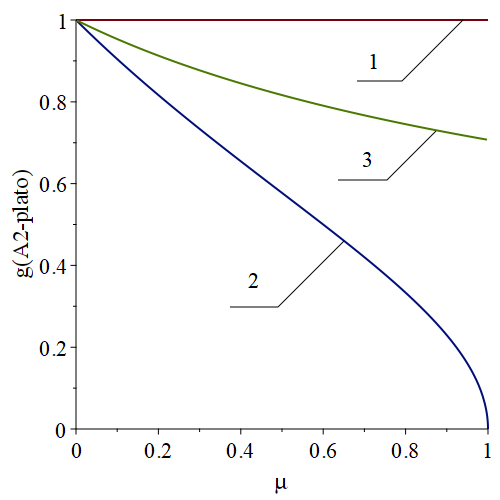
\includegraphics[width=0.8\textwidth]{Eq_tochki_plato_A2.png}
		\caption{Nodal frequencies $g_l$, $g_c$ and intermediate point $g_{1/2}$ depending on mass ratio coefficient $\mu$. 1 ---nodal frequency $g_c=1$, 2 --- left nodal frequency $g^2_l=(1+\mu)/(1+\mu)$, 3 --- intermediate frequency $g^2_{1/2}=1/(1+\mu)$ }
		\label{fig:Eq_tochki_plato_A2}
	\end{figure}
	
	
	Required coefficient $\gamma_{1/2}$ is found from condition:
	\begin{equation}
		A_2(g_{1/2})=\frac{1}{\mu},
		\label{eq:uslovf21}
	\end{equation}
	\begin{equation}
		f^2=\frac{1-\mu}{(1+\mu)^2}.
		\label{eq:uslovf22}
	\end{equation}
	
	Considering \eqref{eq:uslovf21}, \eqref{eq:uslovf22}, critical viscous friction coefficient $\gamma_{1/2}$ is:
	\begin{equation}
		\gamma^{2}_{1/2} = 
		\frac{2 \mu -\mu^{2} }{4 \left(\mu+1\right)^{3}}.
	\end{equation}
	
	For coefficient $\gamma_{1/2}$, amplitude-frequency characteristic passes through three points with same ordinate \eqref{eq:uslovf21}. This approach can be extended to amplitude-frequency characteristic passing through three points where central point ordinate differs from two adjacent points:
	\begin{equation}
		A_2(g_l) (1+\varepsilon)=A_2(g_{\text{1/2}}(\varepsilon)) =A_2(g_c) (1+\varepsilon)
		\label{eq:eqa2lc}
	\end{equation}
	
	Extended problem~\eqref{eq:eqa2lc} has solution:
	
	\begin{equation}
		(\gamma_{1/2} \left(\varepsilon\right))^{2} = 
		\frac{2 \mu -\mu^{2} }{4 \left(\mu+1\right)^{3}}+\frac{\varepsilon}{2 \left(\mu+1\right)^{3}}+\frac{\varepsilon^{2}}{4 \left(\mu +1\right)^{3}}
	\end{equation}
	
	Coefficient $\gamma_{1/2}(\varepsilon)$ can serve as tuning parameter allowing increase/decrease of mass $m_2$ oscillation amplitudes relative to vertical nodal point positions.
	
	To demonstrate presented dynamic mode, Fig.~\ref{fig:a2_mu1} shows amplitude-frequency characteristics with fixed coefficient $\mu=0.1$, reflecting dynamic features of vibrational absorber oscillations for various $\gamma(\varepsilon)$ damping coefficients, where $\varepsilon = -0.02 .. 0.02, 0.01$. 
	
	\begin{figure}[H]
		\centering
		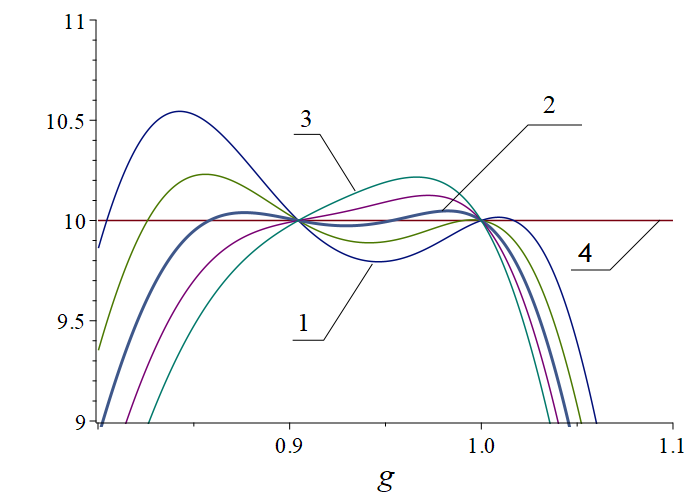
\includegraphics[width=0.8\textwidth]{a2}
		\caption{Amplitude-frequency characteristic family $|A_2(g)|$ for dynamic absorber mode ($\mu = 0.1$, $f = 0.91$) with various damping coefficients $\gamma(\varepsilon)$, where $\varepsilon = -0.02 \ldots 0.02$ with step $0.01$; curve 1 --- $\varepsilon = -0.02$ (local oscillation amplitude reduction), curve 2 --- $\varepsilon = 0$ (critical damping, three-point plateau), curve 3 --- $\varepsilon = 0.02$ (local oscillation amplitude intensification), horizontal line 4 --- level $1/\mu = 10$ (nodal point heights $g_l$ and $g_c$)}
		\label{fig:a2_mu1}
	\end{figure}
	
	
	
	All curves intersect at two nodal points: left $g_l$ and central $g_c$, with coordinates independent of damping coefficient $\gamma$. Curve 2 ($\varepsilon = 0$) demonstrates three-point plateau formation based on points $g_l$, $g_{1/2}$ and $g_c$, ensuring stable $m_2$ oscillation amplitude in specified frequency range. Curves 1 and 3 show amplitude control possibility through parameter $\varepsilon$: reduction (curve 1) or increase (curve 3) of amplitude at intermediate frequency $g_{1/2}$ relative to plateau level.
	
	Fig.~\ref{fig:a2_mu09} illustrates $X_2$ coordinate oscillation dynamics for mass coefficient $\mu = 0.9$, close to unity, characteristic of resonant vibrational test stands where working organ mass is comparable to vibrator mass. 
	
	\begin{figure}[H]
		\centering
		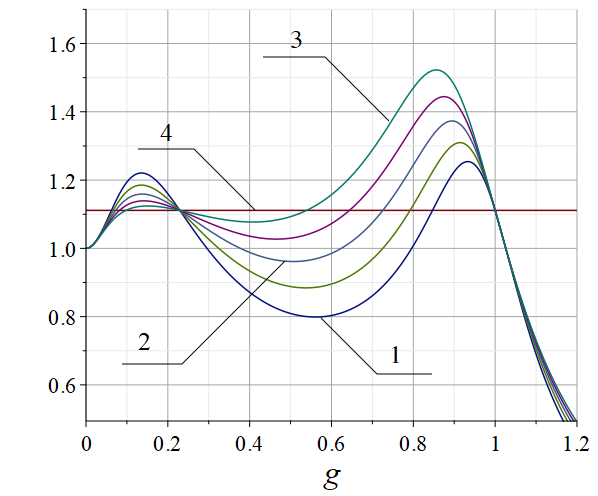
\includegraphics[width=0.8\textwidth]{a2mu09}
		\caption{Amplitude-frequency characteristic family $|A_2(g)|$ for fixed coefficient $\mu = 0.9$ with various damping coefficients $\gamma(\varepsilon)$, where $\varepsilon = -0.02 .. 0.02, 0.01$; lines 1 --- $\varepsilon = -0.02$, lines 2 --- $\varepsilon = 0$, lines 1 --- $\varepsilon = 0.02$, lines 4 --- level $\frac{1}{\mu}$}
		\label{fig:a2_mu09}
	\end{figure}
	
	Compared to Fig.~\ref{fig:a2_mu1} ($\mu = 0.1$), significant change in amplitude-frequency characteristic shape is observed: central peak height decreases to $1/\mu \approx 1.11$, while distance between invariant points $g_l$ and $g_r$ decreases. Three-point plateau (curve 2) becomes less pronounced, indicating increased system sensitivity to excitation frequency changes. Nevertheless, proposed $\gamma_{1/2}(\varepsilon)$ tuning method effectively controls working organ amplitude near resonance zone.
	
	Fig.~\ref{fig:A2_platoA2} shows amplitude-frequency characteristic values at three-point plateau intermediate point depending on mass ratio coefficient $\mu$ for various $\varepsilon$ values.
	
	\begin{figure}[H]
		\centering
		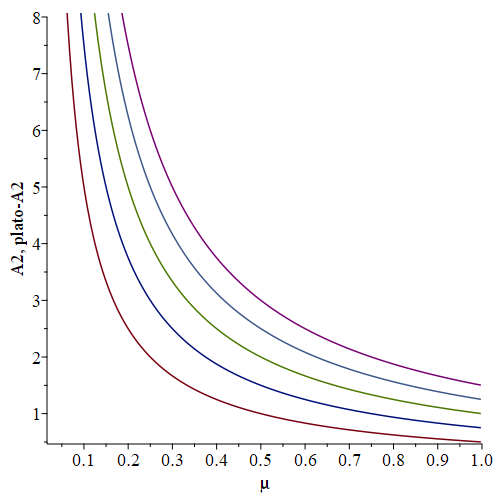
\includegraphics[width=0.8\textwidth]{A2_platoA2.png}
		\caption{Amplitude-frequency characteristic family}
		\label{fig:A2_platoA2}
	\end{figure}
	
	
	Fig.~\ref{fig:A1_platoA2} shows amplitude-frequency characteristic $A_1$ values at three-point plateau intermediate point implemented for $A_2$, depending on mass ratio coefficient for various $\varepsilon$ values.
	
	\begin{figure}[H]
		\centering
		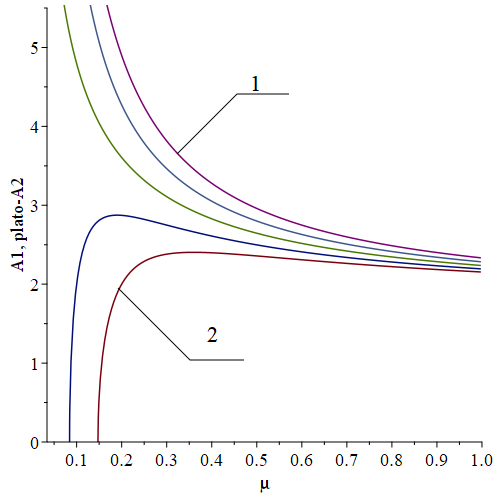
\includegraphics[width=0.8\textwidth]{A1_platoA2.png}
		\caption{Amplitude-frequency characteristic $A_1$ values at intermediate frequency for $A_2$ - plateau. 1 --- monotonic decrease depending on $\mu$; 2 --- dependency on $\mu$ with extremum. $\varepsilon = -0.2 .. 0.2, 0.10$ }
		\label{fig:A1_platoA2}
	\end{figure}
	
	Specifically, graphs in Fig.~\ref{fig:A1_platoA2} show that amplitude-frequency characteristic dependency feature significantly depends on intensity coefficient $\varepsilon$.
	
	Additional interest represents dynamic quality evaluation for free mass generalized coordinate constructed based on two amplitude-frequency characteristics. 
	
	\section*{IX. Dependency of Amplitude-Frequency Characteristics Ensuring $A_2$-Plateau Depending on Coefficient $\mu$ }
	
	Figs.~\ref{fig:mu01}-~\ref{fig:mu10} show pairs of amplitude-frequency characteristics reflecting oscillation dynamic quality (absorber/working organ) with amplitude-frequency characteristic in three-point plateau form.
	
	\begin{figure}[H]
		\centering
		\begin{minipage}{0.45\textwidth}
			\centering
			\includegraphics[width=\textwidth]{platoA2mu01.eps}
			\caption{\(\mu = 0.1\)}
			\label{fig:mu01}
		\end{minipage}\hfill
		\begin{minipage}{0.45\textwidth}
			\centering
			\includegraphics[width=\textwidth]{platoA2mu02.eps}
			\caption{\(\mu = 0.2\)}
			\label{fig:mu02}
		\end{minipage}
	\end{figure}
	
	\begin{figure}[H]
		\centering
		\begin{minipage}{0.45\textwidth}
			\centering
			\includegraphics[width=\textwidth]{platoA2mu03.eps}
			\caption{\(\mu = 0.3\)}
			\label{fig:mu03}
		\end{minipage}\hfill
		\begin{minipage}{0.45\textwidth}
			\centering
			\includegraphics[width=\textwidth]{platoA2mu04.eps}
			\caption{\(\mu = 0.4\)}
			\label{fig:mu04}
		\end{minipage}
	\end{figure}
	
	\begin{figure}[H]
		\centering
		\begin{minipage}{0.45\textwidth}
			\centering
			\includegraphics[width=\textwidth]{platoA2mu05.eps}
			\caption{\(\mu = 0.5\)}
			\label{fig:mu05}
		\end{minipage}\hfill
		\begin{minipage}{0.45\textwidth}
			\centering
			\includegraphics[width=\textwidth]{platoA2mu06.eps}
			\caption{\(\mu = 0.6\)}
			\label{fig:mu06}
		\end{minipage}
	\end{figure}
	
	\begin{figure}[H]
		\centering
		\begin{minipage}{0.45\textwidth}
			\centering
			\includegraphics[width=\textwidth]{platoA2mu07.eps}
			\caption{\(\mu = 0.7\)}
			\label{fig:mu07}
		\end{minipage}\hfill
		\begin{minipage}{0.45\textwidth}
			\centering
			\includegraphics[width=\textwidth]{platoA2mu08.eps}
			\caption{\(\mu = 0.8\)}
			\label{fig:mu08}
		\end{minipage}
	\end{figure}
	
	\begin{figure}[H]
		\centering
		\begin{minipage}{0.45\textwidth}
			\centering
			\includegraphics[width=\textwidth]{platoA2mu09.eps}
			\caption{\(\mu = 0.9\)}
			\label{fig:mu09}
		\end{minipage}\hfill
		\begin{minipage}{0.45\textwidth}
			\centering
			\includegraphics[width=\textwidth]{platoA2mu10.eps}
			\caption{\(\mu = 1.0\)}
			\label{fig:mu10}
		\end{minipage}
	\end{figure}
	
	Key feature of these mode manifestations is mass ratio coefficient limitation by unity $\mu < 1$. Specifically, graphs show that for small mass coefficients $\mu < 1$, generalized coordinate $X_2$ oscillation amplitudes significantly exceed $X_1$ coordinate oscillation amplitudes, with amplitude becoming sensitive to excitation frequency changes. As mass coefficient $\mu$ increases, $X_2$ coordinate amplitude becomes smaller than $X_1$ oscillation amplitude. Critical coefficient is $\mu=1/3$.
	
	Intersection point determination is shown in graph~\ref{fig:perA1A1platoA2}.
	Mass ratio is found by solving equation:
	\begin{equation}
		\frac{3 \mu^{2}+2 \mu}{\mu^{2}} = 
		\frac{1}{\mu^{2}}.
	\end{equation}
	
	Critical ratio is $\mu=1/3$.
	
	\begin{figure}[H]
		\centering
		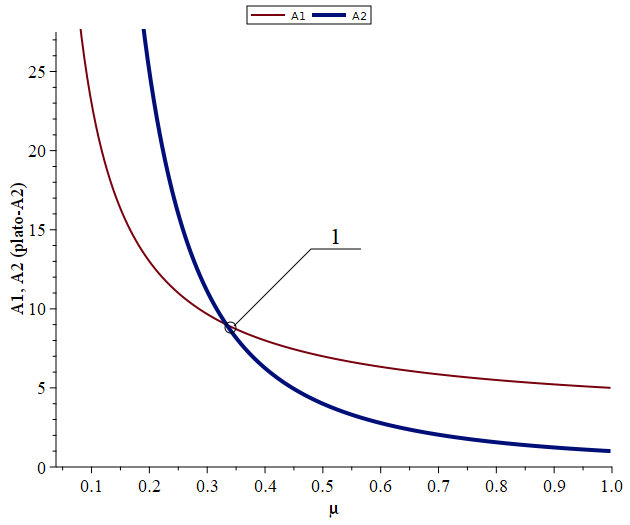
\includegraphics[width=0.8\textwidth]{perA1A1platoA2.png}
		\caption{Intersection point determination of amplitude-frequency characteristics $A_1$ and $A_2$ for $A_2$-plateau condition.}
		\label{fig:perA1A1platoA2} 
	\end{figure}
	
	Main features of amplitude-frequency characteristic mutual arrangement are that mass coefficient change provides two different modes: plateau may exceed or be below second amplitude-frequency characteristic at intermediate frequency. Boundary mass coefficient value is $\mu=1/3$.
	
	Thus, for $\mu < 1/3$, vibrational machine can be considered operating in effective resonance mode. Efficiency condition can be tightened by requiring amplitude-frequency characteristic maxima to be in specified ratio. Question arises about system parameter selection simultaneously ensuring plateau for two amplitude-frequency characteristics. 
	
	However, it can be shown that plateau for two coordinates simultaneously is not implementable.
	
	\section*{X. Incompatibility of $A_2$-Plateau and $A_1$-Plateau Implementation Modes}
	
	Modes ensuring "plateau" for coordinates $X_1$ and $X_2$ are incompatible because implementation conditions 
	\begin{equation}
		f = \frac{1}{1+\mu}, f^2 = \frac{1-\mu}{(1+\mu)^2}  
	\end{equation}	
	have no intersection points. Fig.~\ref{fig:fm} shows graphs depicting variable $f$ relationships with $\mu$ ensuring nodal point ordinate equality conditions for amplitude-frequency characteristics $A_1$ and $A_2$. Curves 1 and 2 don't intersect, demonstrating impossibility of simultaneous pairwise nodal equality for amplitude-frequency characteristics $A_1$ and $A_2$.
	
	\begin{figure}[H]
		\centering
		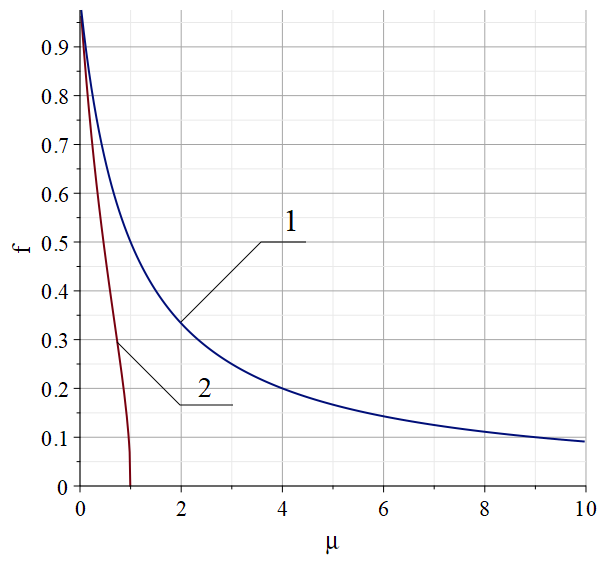
\includegraphics[width=0.8\textwidth]{fmu.png}
		\caption{Curves ensuring nodal height equality: 1 --- nodal ordinate equality condition for $A_1$ as $f= 1/(1+\mu)$ ; 2 --- nodal ordinate equality condition for $g_l$ and $g_c$ for $A_2$ as $f^2 = (1-\mu)/(\mu +1)^2 $} 
		\label{fig:fm}
	\end{figure}
	
	Thus, two strategies can be conditionally implemented for forming dynamic quality of vibrational technological machine elements: ensuring "plateau" for first generalized coordinate $X_1$ ($A_1$-plateau), ensuring plateau for generalized coordinate $X_2$ ($A_1$-plateau).
	
	It can be assumed that two simultaneous plateaus condition exists, but only for systems with higher degrees of freedom, or when adding motion transformation device to oscillatory system.
	
	\section*{XI. Amplitude-Frequency Characteristic of Inter-Partial Connection Transfer Function}
	
	As inter-partial connection transfer function, consider ratio of generalized coordinate oscillation amplitudes:
	\begin{equation}
		W_{12} = \frac{X_1}{X_2}.
	\end{equation}
	Based on structural diagram, transfer function can be obtained as: 	
	\begin{equation}
		W_{12}(j\omega) = \frac{X_1}{X_2} = \frac{k_2 - m_2\omega^2 + j\omega c_2}{k_2 + j\omega c_2}.
	\end{equation}
	In dimensionless form, inter-partial connection transfer function amplitude-frequency characteristic is:
	\begin{equation}
		W_{12}(g) = \frac{1 - (g/f)^2 + 2 j\gamma(g/f)}{1 +2 j\gamma(g/f)}.
		\label{eq:W12}
	\end{equation}
	
	Inter-partial connection transfer function amplitude-frequency characteristic in dimensionless form is:
	
	\begin{equation}
		A_{12}^{2} = 
		\frac{f^{4}-2 f^{2} g^{2}+g^{4}+4 \gamma^{2} g^{2}}{f^{4}+4 \gamma^{2} g^{2}}.
	\end{equation}
	
	Note that $A_{12}$ doesn't explicitly depend on mass ratio. 
	
	Use nodal point determination method based on limiting values $\gamma = 0$ and $\gamma \to \infty$. If $\gamma = 0$ (no damping), limiting amplitude-frequency characteristic is:
	\begin{equation}
		|A_{12}|_{\gamma=0} = \left|1 - \left(\frac{g}{f}\right)^2\right|.
		\label{eq:A12_gamma0}
	\end{equation}
	
	If $\gamma \to \infty$ (infinite damping), limiting amplitude-frequency characteristic is:
	\begin{equation}
		|A_{12}|_{\gamma\to\infty} = 1.
		\label{eq:W12_gammainf}
	\end{equation}
	
	Equality of corresponding amplitude-frequency characteristic moduli defines condition for existence of nodal point independent of $\gamma$:
	\begin{equation}
		|A_{12}|_{\gamma=0} = |A_{12}|_{\gamma\to\infty}.
		\label{eq:W12_node_condition}
	\end{equation}
	
	Substituting \eqref{eq:A12_gamma0} and \eqref{eq:W12_gammainf} into \eqref{eq:W12_node_condition}:
	\begin{equation}
		\left|1 - \left(\frac{g}{f}\right)^2\right| = 1.
		\label{eq:W12_equation}
	\end{equation}
	
	Roots of equation \eqref{eq:W12_equation} are frequencies:
	\begin{align}
		1 - \left(\frac{g}{f}\right)^2 &= 1 \quad \Rightarrow \quad g = 0, \label{eq:node1} \\
		1 - \left(\frac{g}{f}\right)^2 &= -1 \quad \Rightarrow \quad g = f\sqrt{2}. \label{eq:node2}
	\end{align}
	
	Non-trivial solution of equation \eqref{eq:W12_equation} is only one frequency; inter-partial connection amplitude-frequency characteristic $A_{12}$ equals unity:
	\begin{equation}
		g = f\sqrt{2}, |A_{12}|_{	g = f\sqrt{2}} = 1.
		\label{eq:W12_node_final}
	\end{equation}
	
	Fig.~\ref{fig:a12_mu01} shows inter-partial transfer function $W_{12}(g)$, characterizing oscillation amplitude ratio of coordinate $X_1$ and coordinate $X_2$ depending on dimensionless frequency $g$.
	
	
	\begin{figure}[H]
		\centering
		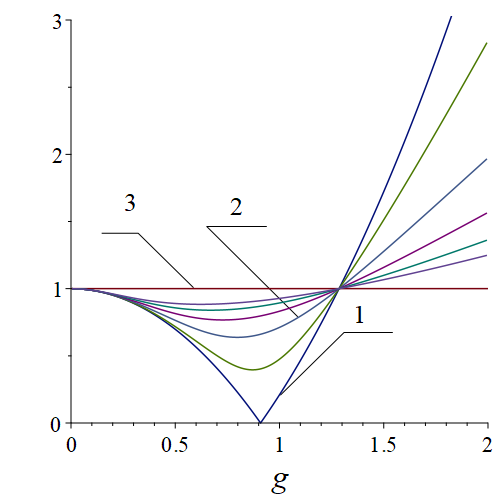
\includegraphics[width=0.8\textwidth]{A12_1m01.png}
		\caption{Inter-partial connection amplitude-frequency characteristic family $|A_{12}(g)| = |X_1/X_2|$ with various damping coefficients $\gamma = 0 \ldots 1$ with step $0.2$; curve 1 --- no damping ($\gamma = 0$), curves 2 --- $\gamma > 0$, horizontal line 3 --- level $|A_{12}| = 1$ (nodal point ordinate)}
		\label{fig:a12_mu01} 
	\end{figure}	
	
	
	
	Important feature of this characteristic is explicit independence from mass ratio $\mu$, making it universal diagnostic tool. Curves intersect at nodal point $g = f\sqrt{2}$, where $|A_{12}| = 1$ (oscillation amplitudes of coordinates $X_1$ and $X_2$ are equal regardless of damping). For $g < f\sqrt{2}$, $|A_{12}| < 1$ (coordinate $X_1$ oscillation amplitude smaller than coordinate $X_2$ oscillation amplitude), for $g > f\sqrt{2}$ --- $|A_{12}| > 1$ (coordinate $X_1$ oscillation amplitude larger than coordinate $X_2$ oscillation amplitude). Nodal point presence enables parameter-free diagnostics: measuring frequency where $|X_1| = |X_2|$, tuning parameter $f$ can be estimated without knowing $\mu$ and $\gamma$.
	
	Consider how inter-partial connection amplitude-frequency characteristic $A_{12}$ looks depending on selected "plateau" conditions. If "plateau" is implemented for amplitude-frequency characteristic $A_1$, then for constructing inter-partial connection amplitude-frequency characteristic, consider:
	
	\begin{equation}
		f = \frac{1}{\mu+1}, \\
		\gamma^{2} = 
		\frac{\mu}{2 \left(\mu  +1\right)^{3}}.
	\end{equation}
	
	In this case, inter-partial connection amplitude-frequency characteristic explicitly depends on mass ratio parameter $\mu$ :
	
	\begin{equation}
		{A_{12}^2}_{(A_1-plato)}=\frac{1-2\left( \mu  + 1 \right) g^{2} + \left(\mu   +1\right)^{4} g^{4}}{1+\left(2 \mu^{2}+2 \mu \right) g^{2}}.
	\end{equation}
	
	
	Fig.~\ref{fig:a12_p1_m0110} illustrates inter-partial characteristic evolution with mass ratio $\mu$ varying widely from $0.01$ (light absorber) to $10$ (heavy vibrator test stand working organ). For each configuration, critical damping coefficient $\gamma_{\text{cr}}$ ensuring three-point plateau for primary mass $m_1$ is selected.
	
	\begin{figure}[H]
		\centering
		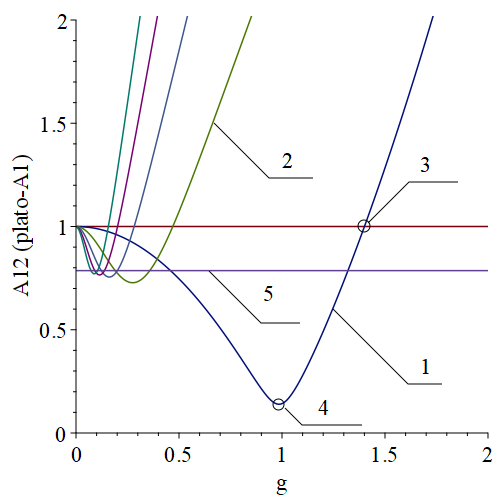
\includegraphics[width=0.8\textwidth]{a12_p1_m0110.png}
		\caption{Inter-partial connection amplitude-frequency characteristic family $|A_{12}(g)|$ ($A_1$ plateau) for critical friction coefficient with various $\mu =  0.01..10,2$; 1 --- $\mu=0.01$, 2 --- $0.01<\mu<10$, 3 -- critical point, 4 -- extremal point, 5 -- limiting level.} 
		\label{fig:a12_p1_m0110}
	\end{figure}
	
	
	Special frequency where amplitude-frequency characteristic crosses unity level is critical value: 
	\begin{equation}
		g_{cr}=\frac{\sqrt{2}}{\mu   +1}.
	\end{equation}
	
	
	Another feature is presence of frequency where amplitude-frequency characteristic has extremum - local minimum. In this case,
	stationary point is frequency:
	
	\begin{equation}
		g_{st}^2=\frac{-\mu -1+\sqrt{5 \mu ^{2}+6 \mu +1}}{2 \left(\mu ^{2}+2\mu +1\right) \mu}.
	\end{equation}
	
	
	\begin{figure}[H]
		\centering
		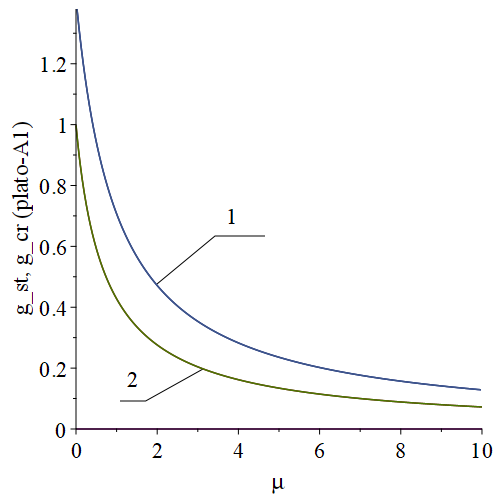
\includegraphics[width=0.8\textwidth]{g_st_mu_A1plato.png}
		\caption{Dependency of stationary and critical frequencies for inter-partial connection amplitude-frequency characteristic on $\mu$. 1 --- critical frequency, 2 --- stationary frequency} 
		\label{fig:g_st_mu_A1plato}
	\end{figure}
	
	Limiting values are:
	
	\begin{equation}
		\lim_{\mu\to 0} 	g_{st}=1
	\end{equation}
	
	and
	
	\begin{equation}
		\lim_{\mu\to \infty} 	g_{st}=0
	\end{equation}
	
	
	Extreme inter-partial connection amplitude-frequency characteristic value is 
	
	\begin{equation}
		A_{12}^2(g_{st})=\frac{\left(-\mu^{2}-4 \mu -1\right) \sqrt{5 \mu^{2}+6 \mu +1}+5 \mu ^{3}+11 \mu^{2}+7 \mu +1}{2\mu^{2} \sqrt{5 \mu^{2}+6 \mu +1} }
	\end{equation}
	
	\begin{figure}[H]
		\centering
		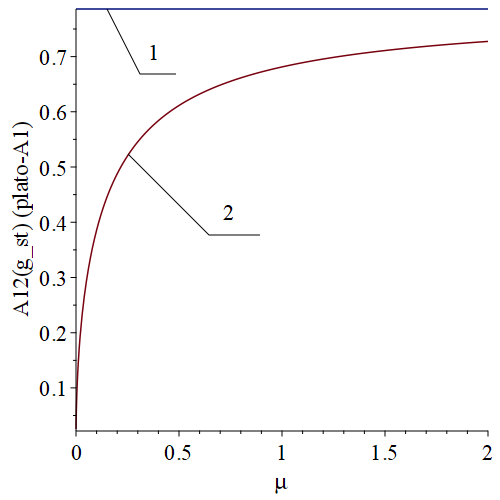
\includegraphics[width=0.8\textwidth]{A12_g_st_mu_A1plato.png}
		\caption{Dependency of inter-partial connection amplitude-frequency characteristic calculated at stationary frequency $g_{st}$ depending on $\mu$. 1 --- limiting value 2 --- extreme amplitude-frequency characteristic value} 
		\label{fig:A12_g_st_mu_A1plato}
	\end{figure}
	
	
	
	
	Limiting values are:
	
	\begin{equation}
		\lim_{\mu\to 0} 	A_{12}(g_{st})=0
	\end{equation}
	
	and
	
	\begin{equation}
		\lim_{\mu\to \infty } 	A_{12}(g_{st})=\sqrt{-\frac{1}{2}+\frac{\sqrt{5}}{2}}
	\end{equation}
	
	
	
	If "plateau" is implemented for amplitude-frequency characteristic $A_2$, then for constructing inter-partial connection amplitude-frequency characteristic, consider analogous conditions:
	
	
	\begin{equation}
		f^2 = \frac{1-\mu}{\left(\mu +1\right)^{2}}, \quad 
		\gamma^{2} = 
		\frac{-\mu^{2}+2 \mu}{4 \left(\mu+1\right)^{3}}, \quad 
		\mu \le 1.
	\end{equation}
	
	Corresponding inter-partial connection amplitude-frequency characteristic will be: 
	
	\begin{equation}
		{A_{12}^{2}}_{(A_2-plato)} = 
		\frac{\left(-\mu^{2}+2 \mu\right) \mu^{2} g^{2} \left(\mu+1\right)+\left(\left(1-\mu\right) \mu-g^{2} \mu\left(\mu +1\right)^{2}\right)^{2}}{\left(1-\mu\right)^{2} \mu^{2}+{\left(-\mu^{2}+2 \mu\right) \mu^{2} g^{2}\left(\mu+1\right)}}.
	\end{equation}	
	
	
	Fig.~\ref{fig:a12_p2_m011} shows inter-partial connection characteristics for absorber mass $m_2$ (working organ) plateau formation mode, where tuning parameter is determined from condition $f^2 = (1-\mu)/(1+\mu)^2$, and damping --- from three-point contact condition $\gamma_{1/2}$. 
	
	\begin{figure}[H]
		\centering
		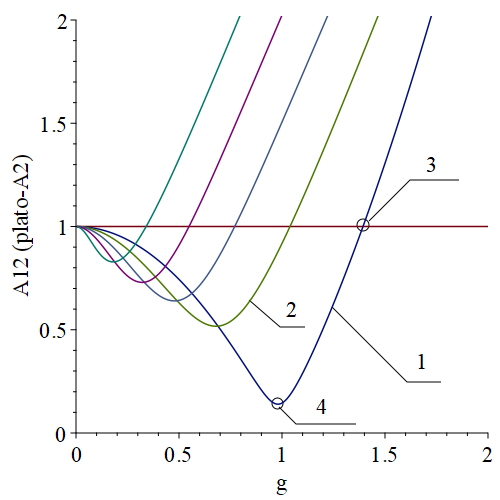
\includegraphics[width=0.8\textwidth]{a12_p2_m011.png}
		\caption{Inter-partial connection amplitude-frequency characteristic family $|A_{12}(g)|$ ($X_2$ plateau) for critical friction coefficient with various $\mu =  0.01..1,0.2$; 1 --- $\mu=0.01$, 2 --- $0.01<\mu<1$, 3 -- critical point, 4 -- extremal point } 
		\label{fig:a12_p2_m011}
	\end{figure}
	
	
	Special frequency where amplitude-frequency characteristic crosses unity level is critical value: 
	\begin{equation}
		g_{cr}=\frac{\sqrt{2-2 \mu}}{\mu +1}
	\end{equation}	
	
	
	Another feature is presence of frequency where amplitude-frequency characteristic has extremum - local minimum, which is also global minimum. In this case,
	stationary point is frequency:
	
	\begin{equation}
		g_{st}^2=\frac{\left(-1+\mu   \right) \left(\mu ^{2}+\sqrt{3 \mu ^{4}-4 \mu ^{3}-4 \mu ^{2}+4 \mu   +1}-1\right)}{\mu ^{4}-3 \mu ^{2}-2 \mu  }
	\end{equation}
	
	
	
	
	\begin{figure}[H]
		\centering
		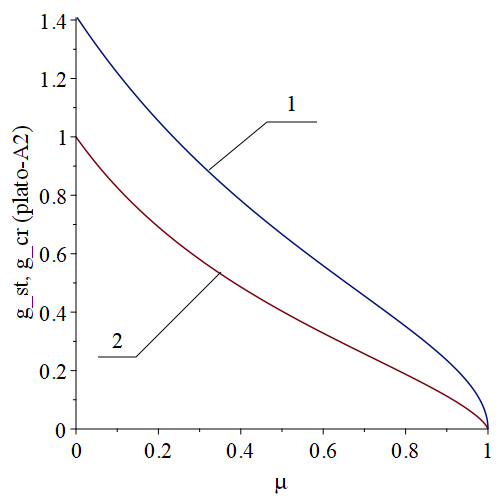
\includegraphics[width=0.8\textwidth]{g_st_mu_A2plato.png}
		\caption{Dependency of stationary frequency for inter-partial connection amplitude-frequency characteristic depending on $\mu$. 1 --- critical frequency, 2 --- stationary frequency} 
		\label{fig:g_st_mu_A2plato}
	\end{figure}
	
	
	Limiting values are:
	
	\begin{equation}
		\lim_{\mu\to 0} 	g_{st}=1
	\end{equation}
	
	and
	
	\begin{equation}
		\lim_{\mu\to \infty} 	g_{st}=0
	\end{equation}
	
	Extreme inter-partial connection amplitude-frequency characteristic value is 
	
	\begin{equation}
		A_{12}^2(g_{st})=\frac{\left(-1+\mu  \right) \left(\mu ^{2}+\sqrt{3 \mu ^{4}-4 \mu ^{3}-4 \mu ^{2}+4 \mu   +1}-1\right)}{\mu ^{4}-3 \mu ^{2}-2 \mu }
	\end{equation}	
	
	
	
	\begin{figure}[H]
		\centering
		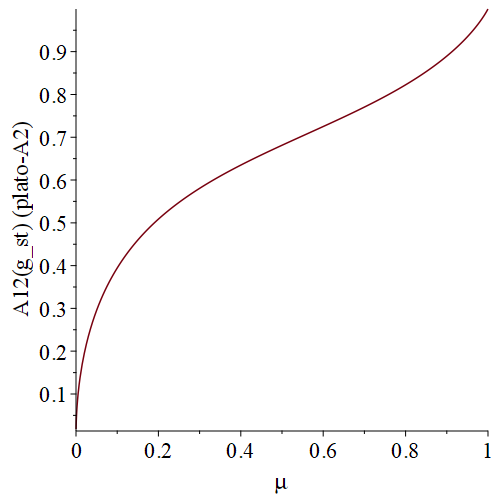
\includegraphics[width=0.8\textwidth]{A12_g_st_mu_A2plato.png}
		\caption{Dependency of inter-partial connection amplitude-frequency characteristic calculated at stationary frequency $g_st$ depending on $\mu$} 
		\label{fig:A12_g_st_mu_A2plato}
	\end{figure}
	
	
	Fig.~\ref{fig:a12_2m01} shows inter-partial connection $A_{12}$ behavior with special tuning parameter $f$ ensuring amplitude equality at left and central invariant points of system $A_2$ amplitude-frequency characteristic ($A_2(g_l) = A_2(g_c) = 1/\mu$). This configuration corresponds to optimal mode of coordinate $X_2$ mass $m_2$ oscillation amplitude plateau formation.
	
	
	For each plateau, either for $A_1$ or for $A_2$, corresponding inter-partial connection amplitude-frequency characteristic can be constructed. 
	
	Assume $A_1$ plateau conditions are implemented, then amplitude-frequency characteristics are:
	
	\begin{equation}
		A^2_1(A_1-plato) = \frac{\mu  +2}{\mu }, 	 \quad 	A^2_2(A_1-plato) = \frac{2 \mu  +1}{\mu^{2}}.
	\end{equation}
	
	Corresponding inter-partial connection amplitude-frequency characteristic $A_{12}$ under $A_1$-plateau condition is:
	\begin{equation}
		\frac{A^2_1}{A^2_2}(A_1-plato)=\frac{(\mu+2)\mu}{2 \mu  +1 }.
	\end{equation}
	
	If vibration intensity correction coefficient $\varepsilon$ is fixed, corresponding amplitude-frequency characteristics $A_1(\varepsilon)$ and $A_2(\varepsilon)$ can be calculated considering corresponding friction coefficient $\gamma(\varepsilon)$:
	
	\begin{equation}
		A^2_1(\varepsilon)_{A_{1}-plato} = 
		\frac{\left(1+\varepsilon \right)^2 \left(\mu  +2\right)}{\mu} ,
	\end{equation}
	\begin{equation}
		A^2_2(\varepsilon)_{A_{1}-plato} = 
		\frac{1+\left(\varepsilon^{2}+2 \varepsilon\right) \mu^{2}+2 \left(1+\varepsilon\right)^{2} \mu}{\mu^{2}}.
	\end{equation}
	Corresponding $A_1$-plateau inter-partial connection amplitude-frequency characteristic, considered as function of parameter $\varepsilon$, is:
	\begin{equation} 
		{A_{12}^2} \! (\varepsilon)_{A_{1}-plato} = 
		\frac{\left(1+\varepsilon\right)^{2}\left(\mu+2\right)\mu}{1+\left(\varepsilon^{2}+2 \varepsilon \right) \mu^{2}+2 \left(1+\varepsilon\right)^{2} \mu}.
	\end{equation}	
	
	Fig.~\ref{fig:A1exper_a1_plato} shows amplitude-frequency characteristic family for various vibration "deformation" coefficients depending on mass ratio coefficient $\mu$. Specifically, graph family is combined with experimental test results of laboratory vibrational test stand with various mass and stiffness coefficients. Presented combination of experimental data with analytical dependencies can be considered as algorithm for determining modes ensuring $A_{1}$-plateau implementation with minimal $\varepsilon$-deviation.
	
	Now consider $A_2$ plateau conditions. In this case, amplitude-frequency characteristics are:
	
	\begin{equation}
		A^2_2(\mu)_{A_2-plato} = 	\frac{1}{\mu^{2}}, \quad
		A^2_1(\mu)_{A_2-plato} = 	\frac{3 \mu +2}{\mu }.
	\end{equation}	
	
	Corresponding $A_{2}$-plateau inter-partial connection amplitude-frequency characteristic $A_{12}$ is:
	
	\begin{equation}	
		\frac{A^2_1}{A^2_2}_{A_2-plato} =(3 \mu +2)\mu.
	\end{equation}
	
	For tuning parameter $\varepsilon$, amplitude-frequency characteristics become:
	
	\begin{equation}
		A^2_2(\varepsilon)_{A_2-plato} = 
		\frac{\left(1+\varepsilon  \right)^{2}}{\mu^{2}}
		, \quad
		A^2_1(\varepsilon)_{A_2-plato} = 
		\frac{3 \mu^{2}+\varepsilon^{2}+2 \mu+2 \varepsilon }{\mu^{2}}
	\end{equation}
	
	Corresponding $A_{2}$-plateau inter-partial connection amplitude-frequency characteristic $A_{12}(\varepsilon)$ considering coefficient $\varepsilon$, calculated at frequency $g_{1/2}$, is:
	
	\begin{equation}
		A^2_{12}(\varepsilon)_{A_2-plato} = 
		\frac{3 \mu^{2}+\varepsilon^{2}+2 \mu+2 \varepsilon}{\left(1+\varepsilon\right)^{2}}
	\end{equation}	
	
	Thus, family of inter-partial connection amplitude-frequency characteristic values is obtained considering conditions ensuring $A_2$ plateau.
	
	Fig.\ref{fig:A12_1plato2_data.png} shows combination of theoretical inter-partial connection amplitude-frequency characteristic curves (line 3) and experimental results (areas 1 and 2).
	
	
	
		\begin{figure}[H]
		\centering
		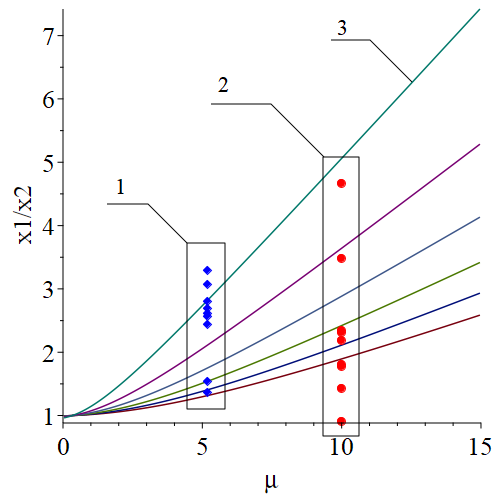
\includegraphics[width=0.8\textwidth]{A12_1plato2_data.png}
		\caption{Combination of theoretical inter-partial connection :  1,2 ----  experimental results; 3 ----  amplitude-frequency characteristic curves } 
		\label{fig:A12_1plato2_data.png}
     	\end{figure}
	
			
	Obviously, inter-partial connection amplitude-frequency characteristic curves for $A_1$ and $A_2$ plateaus are different and can intersect. Find intersection points from conditions: 
	
	\begin{equation}
		A^2_{12}(\varepsilon)_{A_2-plato} = 
		A^2_{12}(\varepsilon)_{A_2-plato}.
		\label{eq:quala12plat1plato2}
	\end{equation}
	
	Expression \ref{eq:quala12plat1plato2} reduces to finding roots of quadratic equation:
	
	\begin{equation}
		\varepsilon^{2}+2 \varepsilon+\frac{6 \mu^{2}}{3\mu^{3}+5 \mu^{2}-3 \mu + 1}
		= 0
	\end{equation}
	
	Equation roots are:
	
	\begin{equation}
		\varepsilon= 
		-1+\sqrt{\frac{3 \mu^{3}-\mu^{2}-3 \mu+1}{3 \mu ^{3}+5 \mu ^{2}-3 \mu+1}},
	\end{equation}
	\begin{equation}
		\varepsilon= 
		-1-\sqrt{\frac{3 \mu^{3}-\mu^{2}-3 \mu+1}{3 \mu ^{3}+5 \mu ^{2}-3 \mu+1}},
	\end{equation}
	
	This dependency between parameters $\varepsilon$ and $\mu$ can be demonstrated in Fig. 
	~\ref{fig:a21eps_mu}
	
	
	\begin{figure}[H]
		\centering
		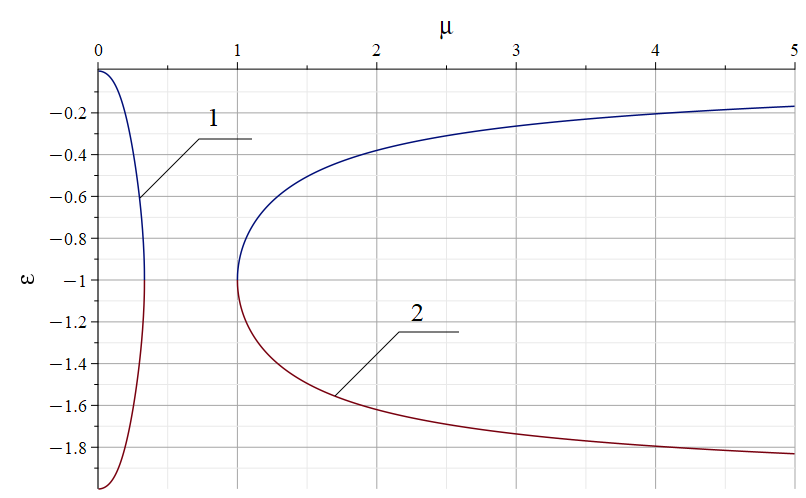
\includegraphics[width=0.8\textwidth]{a21eps_mu.png}
		\caption{Set of $(\varepsilon,\mu)$ pairs ensuring amplitude-frequency characteristic equality for various plateaus} 
		\label{fig:a21eps_mu}
	\end{figure}
	
	
	
	\begin{equation}
		A^2_{12}(\varepsilon)_{A_2-plato} = 
		\frac{3 \mu^{2}+\varepsilon^{2}+2 \mu+2 \varepsilon}{\left(1+\varepsilon\right)^{2}}
	\end{equation}	
	
	
	\begin{equation} 
		{A_{12}^2} \! (\varepsilon)_{A_{1}-plato} = 
		\frac{\left(1+\varepsilon\right)^{2}\left(\mu+2\right)\mu}{1+\left(\varepsilon^{2}+2 \varepsilon \right) \mu^{2}+2 \left(1+\varepsilon\right)^{2} \mu}.
	\end{equation}
	
	
	\begin{figure}[H]
		\centering
		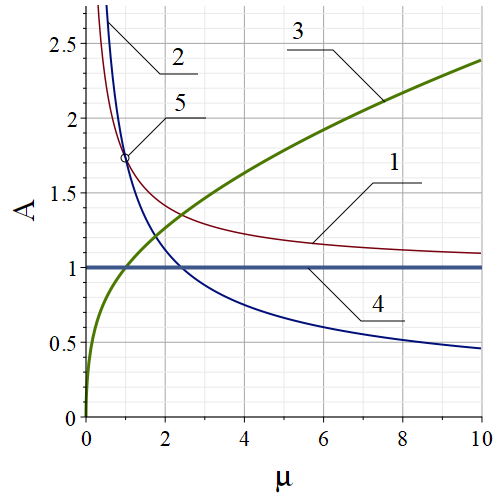
\includegraphics[width=0.8\textwidth]{amplato1.png}
		\caption{} 
		\label{fig:amplato1}
	\end{figure}
	
	\begin{figure}[H]
		\centering
		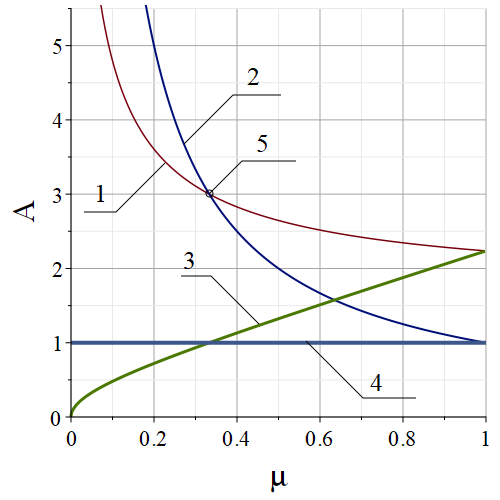
\includegraphics[width=0.8\textwidth]{amplato2.png}
		\caption{} 
		\label{fig:amplato2}
	\end{figure}
	
	
	\begin{figure}[H]
		\centering
		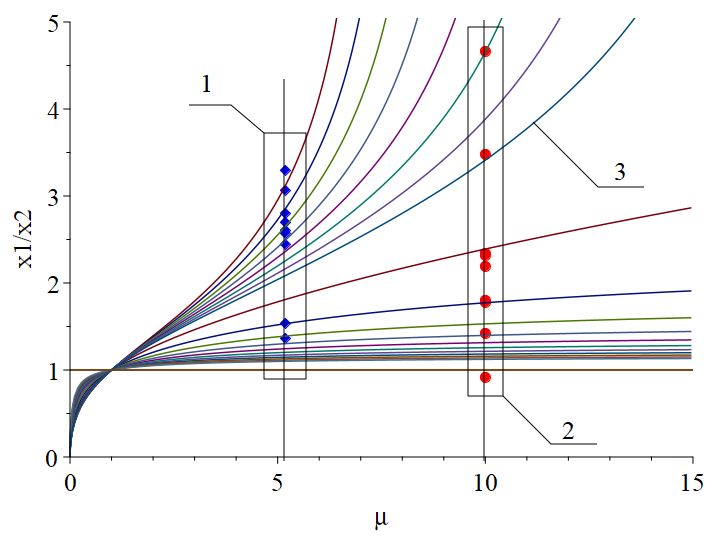
\includegraphics[width=0.8\textwidth]{exper.png}
		\caption{$\varepsilon = - 0.12..1$} 
		\label{fig:A1exper_a1_plato}
	\end{figure}
	
	
	\begin{figure}[H]
		\centering
		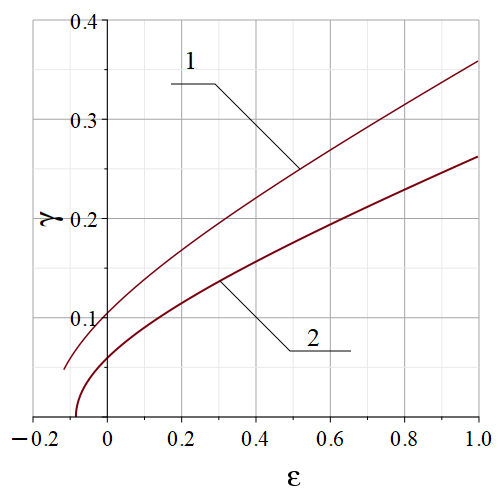
\includegraphics[width=0.8\textwidth]{tren.png}
		\caption{line 1 --- $\mu = 5.18$; line 2 --- $\mu = 10.348$. $\gamma^{2} = 
			\frac{\mu \left(\mu+2\right) \varepsilon^{2}}{4 \left(\mu+1\right)^{3}}+\frac{\mu\left(\mu+2\right) \varepsilon}{2 \left(\mu+1\right)^{3}}+\frac{\mu}{2 \left(\mu +1\right)^{3}}
			$} 
		\label{fig:tren}
	\end{figure}
	
	\begin{figure}[H]
		\centering
		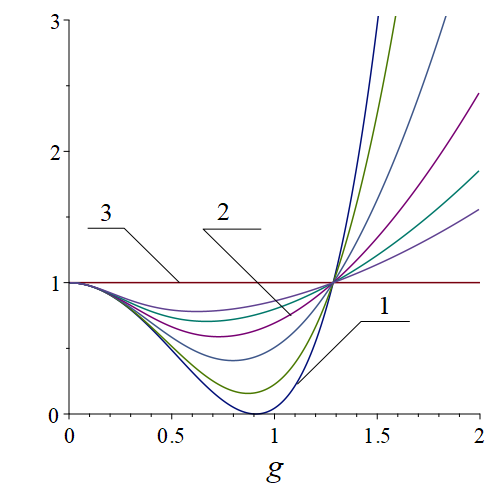
\includegraphics[width=0.8\textwidth]{A12_2m01.png}
		\caption{Inter-partial connection amplitude-frequency characteristic family $|A_{12}(g)|$ for $A_2$ plateau formation ($\mu = 0.1$, $f^2 = (1-\mu)/(1+\mu)^2$) with various damping coefficients $\gamma = 0 \ldots 1$ with step $0.2$; curve 1 --- $\gamma = 0$ (sharp resonance), curves 2 --- $\gamma > 0$ (peak smoothing), horizontal line 3 --- level $|A_{12}| = 1$} 
		\label{fig:a12_2m01}
	\end{figure}
	
	
	% === ЗАКЛЮЧЕНИЕ ===
\section*{Conclusion}

The following results have been obtained in this work:

\begin{enumerate}
	\item Complete analytical expressions for amplitude-frequency characteristics $A_1(g)$ and $A_2(g)$ of a two-mass oscillatory system with viscous damping have been derived.
	
	\item Coordinates of invariant (nodal) points independent of the damping coefficient $\gamma$ have been determined for both partial systems.
	
	\item It has been shown that the condition of equal heights of invariant points for the primary mass leads to the classical Den Hartog tuning $f = 1/(1+\mu)$, while for the working organ it leads to the dependence $f^2 = (1-\mu)/(1+\mu)^2$.
	
	\item Structural invariance of the inter-partial transfer function $W_{12} = X_1/X_2$ has been proved: it does not explicitly depend on the mass ratio $\mu$.
	
	\item It has been shown that the regimes of $A_1$-plateau and $A_2$-plateau are mutually incompatible, as the corresponding tuning conditions have no common solution.
	
	\item An invariant point of the inter-partial connection $g = f\sqrt{2}$ has been found, at which $|W_{12}| = 1$ regardless of the mass ratio and damping coefficient.
\end{enumerate}
	
	% === БЛАГОДАРНОСТИ ===

\section*{Acknowledgments}

The authors express their gratitude to the developers of the Qwen language model for creating tools that assisted in error checking and LaTeX conversion during manuscript preparation.

The structural analysis was supported by the use of the open-source software ``Oscillator Chain Demo'' \cite{EliseevSoftware2026}, developed for interactive demonstration of structural methods for mechanical oscillatory systems.
	
	
	% === БИБЛИОГРАФИЯ ВСТРОЕНА ПРЯМО В ФАЙЛ ===
	\begin{thebibliography}{99}
		
		\bibitem{Kryukov1967}
		Kryukov B.I.
		\textit{Dynamics of resonant-type vibration machines}.
		Kiev: Naukova dumka, 1967. 208 p. [in Russian]
		
		\bibitem{Altschul2022}
		Al'tshul' G.M., Gus'kov A.M., Panovko G.Ya.
		Dynamics of a resonant vibration machine with equal-frequency suspension of the working body and unbalance vibration exciter
		// Ore Beneficiation. 2022. No. 1. P. 51--55. [in Russian]
		
		\bibitem{Panovko2020}
		Panovko G.
		Resonant adjustment of vibrating machines with unbalance vibroexciter. Problems and solutions
		// Smart Innovation, Systems and Technologies. 2020. Vol. 154. P. 51--62.
		
		\bibitem{Eliseev2020}
		Eliseev S.V., Eliseev A.V.
		\textit{Theory of Oscillations: Structural Mathematical Modeling in Problems of Dynamics of Technical Objects}.
		Cham: Springer International Publishing, 2020. 521 p.
		
		\bibitem{Eliseev2023}
		Eliseev A.V.
		\textit{Structural Mathematical Modeling Applications in Technological Machines and Transportation Vehicles}.
		Hershey, PA: IGI Global, 2023. 288 p. DOI: 10.4018/978-1-6684-7237-8
		
		\bibitem{DenHartog1960}
		Den-Gartog Dzh.P.
		\textit{Mechanical Vibrations}.
		Moscow: GIFML, 1960. 580 p. [in Russian]
		
		\bibitem{DenHartog1956}
		Den Hartog J.P.
		\textit{Mechanical Vibrations}. 4th ed.
		New York: McGraw-Hill, 1956.
		
		\bibitem{Svyshch2025}
		Svyshch T.
		Modeling the operation of an eccentric-pendulum resonant vibration stand for testing aviation industry products
		// Vibroengineering Procedia. 2025. Vol. 59. P. 34--40. DOI: 10.21595/vp.2025.25064
		
		\bibitem{Kapalo2025}
		Kapalo R.
		Mathematical modeling of the operation of a resonant vibration stand with an inertial exciter and hydraulic coupling for testing aviation industry products
		// Vibroengineering Procedia. 2025. Vol. 59. P. 28--33. DOI: 10.21595/vp.2025.25059
		
		\bibitem{Lavendel1981}
		Lavendel E.E.
		\textit{Vibrations in Engineering: Vibrational Processes and Machines}. In 6 vol.
		Moscow: Mashinostroenie, 1981. Vol. 4. 509 p. [in Russian]
		
		\bibitem{Eliseev2017}
		Eliseev S.V., Kashuba V.B., Kinash N.Zh.
		Dynamic vibration damping: introduction of additional constraints, lever interactions and physical effects
		// Bulletin of Irkutsk State Technical University. 2017. Vol. 21. P. 10--23. [in Russian]
		
		\bibitem{Lurie}
		Lurie A.I.
		\textit{Analytical Mechanics}.
		Moscow: Fizmatgiz. [in Russian]
		
		\bibitem{Timoshenko1974}
		Timoshenko S.P., Young D.H., Weaver W.
		\textit{Vibration Problems in Engineering}.
		Moscow: Mashinostroenie, 1974. [in Russian]
		
		\bibitem{Nishihara2002}
		Nishihara O., Asami T.
		Parametric optimization of vibration absorbers
		// Journal of Sound and Vibration. 2002. Vol. 253, No. 5. P. 933--955.
		
		\bibitem{Balakhin2008}
		Balakhin O.B.
		\textit{Harmony of Self-Development in Nature and Society: Similarity and Analogies}.
		Moscow: MSU Press, 2008. [in Russian]
		
		\bibitem{EliseevSoftware2026}
		Eliseev A.
		\textit{Oscillator Chain Demo: Interactive Demonstrator of Structural Methods for Mechanical Oscillatory Systems}.
		Version 1.1.0. 2026.
		Available at: \url{https://github.com/poleya/oscillator-chain-demo}.
		DOI: 10.5281/zenodo.21310022.
		
	\end{thebibliography}	
	
\end{document}
